\documentclass[letterpaper,journal]{IEEEtran}
\usepackage{cite}
\usepackage{amsmath,latexsym,amssymb,amsfonts}
\usepackage[utf8]{inputenc}
\usepackage{textcomp}
\usepackage[dvipsnames]{xcolor}
\usepackage{booktabs}
\usepackage{stfloats}
\usepackage{graphicx}
\usepackage{url}
\usepackage{hyperref}
\hypersetup{hidelinks}
\usepackage{bm}
\usepackage{amsthm}

%%%%%%%%%%%%%%%%%%%%%%%%%%%%%%%%%%%%%%%%%%%%%%%%%%%%%%%%%
\usepackage{tikz}
\usetikzlibrary{circuits.ee.IEC}
\usepackage[european resistor, european voltage, european current]{circuitikz}
\usetikzlibrary{arrows, shapes, positioning}
\usetikzlibrary{decorations.markings, decorations.pathmorphing,
decorations.pathreplacing}
\usetikzlibrary{calc,patterns,shapes.geometric}
\usetikzlibrary{shapes.multipart, positioning, patterns, backgrounds}
\tikzstyle{titlebox}=[rectangle,inner sep=10pt,inner ysep=10pt,draw]%
\usetikzlibrary{arrows.meta}
\usetikzlibrary{matrix, fit}

%%%%%%%%%%%%%%%%%%%%%%%%%%%%%%%%%%%%%%%%%%%%%%%%%%%%%%%%%%%%%

\def\blacksquare{\hbox{\vrule width 4pt height 4pt depth 0pt}}
\def\square{\hbox{\vrule width 4pt height 4pt depth 0pt}}
\def\qed{\hfill \square}
\def\qedp{\rightline{$\blacksquare$}}
\def\EXPT{\mathop{{\rm E}}}
\def\MIN{\mathop{{\rm min}}}
\def\MAX{\mathop{{\rm max}}}
\def\LIM{\mathop{{\longrightarrow}}}
\def\UNION{\mathop{\bigcup}}
\def\INTERSECT{\mathop{\bigcap}}
\def\ARGMIN{\mathop{{\rm argmin}}}
\def\ARGMAX{\mathop{{\rm argmax}}}
\def\TOUND{\mathop{\longrightarrow}}
\def\col#1{\mathop{{\rm col}\,\left(\,#1\,\right)}}
\def\rank{\mathop{{\rm rank}}}

\newcommand{\widebox}[2][0.5em]{\fbox{\hspace{#1}$\displaystyle #2$\hspace{#1}}}

% User definition from Shengya
\def\V{\mathcal{V}} % the set of vehicle
\def\E{\mathcal{E}} % the set of edge
\def\G{\mathcal{G}} % graph
\def\A{\mathcal{A}} % adjacency matrix 
\def\W{\mathcal{W}} % weighted adjacency matrix
\def\L{\mathcal{L}} % Laplacian matrix
\def\N{\mathcal{N}} % neighbors
\def\LO{\mathcal{LO}} % the set of observer
\def\DO{\mathcal{DO}} % the set of observer
\def\diag#1{\mathop{{\rm diag}\,\left(\,#1\,\right)}}
\def\ST{\mathcal{ST}} % Self trust
\def\LT{\mathcal{LT}} % Local trust
\def\DT{\mathcal{DT}} % Distributed trust 
\def\VT{\mathcal{VT}} % Vehicle trust 
\def\AT{\mathcal{AT}} % Aggregation trust
\def\T{\mathcal{T}} % Aggregation trust
\def\O{\mathcal{O}} % opinion


% User Defined Color based on RGB
\definecolor{userblue}{RGB}{31,119,180}
\definecolor{userorange}{RGB}{255,127,14}
\definecolor{usergreen}{RGB}{44,160,44}
\definecolor{userpurple}{RGB}{148,103,189}
\definecolor{userred}{RGB}{214,39,40}

\definecolor{blue1}{RGB}{31,119,180}
\definecolor{orange1}{RGB}{255,127,14}
\definecolor{green1}{RGB}{44,160,44}
\definecolor{purple1}{RGB}{148,103,189}
\definecolor{rose1}{RGB}{227, 119, 194}

%%%
\newtheorem{prb}{\it Problem}%[section]
\newtheorem{theorem}{\it Theorem}%[section]
\newtheorem{lemma}{\it Lemma}%[section]
\newtheorem{definition}{\it Definition}
\newtheorem{remark}{\it Remark}%[section]
\newtheorem{assumption}{\it Assumption}%[section]
\newtheorem{example}{\it Example}%[section]
\newtheorem{annex}{\it Annex}%[section]
\newtheorem{prop}{\it Proposition}%[section]

\newtheorem{alert}{\color{red}\it Alert Remark}
% \newtheorem{proof}{\it Proof}%[section]

% Reviewer answers, in ForestGreen.
\newcommand{\azrevcolor}{ForestGreen}
\newcommand{\azrev}[1]{\textcolor{\azrevcolor}{#1}}




\def\BibTeX{{\rm B\kern-.05em{\sc i\kern-.025em b}\kern-.08em
    T\kern-.1667em\lower.7ex\hbox{E}\kern-.125emX}}

\tikzset{global scale/.style={
    scale=#1,
    every node/.append style={scale=#1}
  }
}

\begin{document}
% "Hugues Rafaralahy" <hugues.rafaralahy@univ-lorraine.fr>; 
\title{Trust-Aware Resilient Distributed Observer Design for Connected Vehicle Platoons}
\author{Quang Huy Nguyen, Shengya Meng, Hugues Rafaralahy, Madjid Haddad, Ali Zemouche%
\thanks{This work was supported by SEGULA Engineering. The work of H. Rafaralahy and A. Zemouche was partially supported by the French National Research Agency (ANR) under grant ANR-20-CE48-0015 (ArtISMo project).}%
\thanks{A preliminary version of this work was accepted at the 2026 IFAC World Congress, Busan, South Korea~\cite{nguyen2026ifac}.}%
\thanks{Quang Huy Nguyen, Shengya Meng, Hugues Rafaralahy, and Ali Zemouche are with Universit\'e de Lorraine, CNRS, CRAN, F-57000 Metz, France (e-mail: ali.zemouche@univ-lorraine.fr).}%
\thanks{Quang Huy Nguyen and Madjid Haddad are with SEGULA Engineering, 19 rue d'Arras, 92000 Nanterre, France (e-mail: madjid.haddad@segula.fr).}%
\thanks{QCar/LIMO implementation resources are available at \protect\url{https://github.com/kslhuy/QCar2_Cran}; the demonstration video is available at \protect\url{https://youtu.be/t6-soznp6ks}.}}

\markboth{IEEE Transactions on Intelligent Transportation Systems, 2026}{Nguyen \MakeLowercase{\textit{et al.}}: Trust-Aware Resilient Distributed Observer Design}
\maketitle

\begin{abstract}
This paper develops a trust-aware distributed observer for vehicle platoons described by a discrete-time kinematic bicycle model. Validity and consistency checks produce trust-adaptive weights, while a local-observer anchor prevents drift. Checkable sufficient conditions establish local nonlinear input-to-state stability under bounded model, input, accepted-attack, and switching effects for direct-anchor and sparse accepted graphs. A finite-window rollback mitigates delayed trust decisions and yields a practical ISS bound with an additional reset term. Five-vehicle simulations show suppression of position, speed, and packet-drop attacks. QCar/LIMO tests show reduced post-detection position error and positive path-projected spacing for the tested trust-modulated ACC/CACC scheme.
\end{abstract}

\begin{IEEEkeywords}
Connected and Autonomous Vehicles, system state estimation, methods for security and privacy, distributed observers, trust management.
\end{IEEEkeywords}

\section{Introduction}\label{sec_introduction}
\IEEEPARstart{A}{utonomous} road vehicles are no longer only mechanical platforms with added electronics. Advances in onboard sensing, embedded computation, and AI-supported perception are turning them into mobile cyber-physical systems that process large sensor streams and close control loops in real time. However, single-vehicle autonomy is only one part of the emerging mobility architecture. The next step is cooperation: through vehicle-to-vehicle (V2V) and broader vehicle-to-everything (V2X) communication, multiple vehicles can share state information and coordinate maneuvers, enabling platooning, smoother traffic flow, and safer mobility. In a connected and automated vehicle platoon, each vehicle must estimate not only its own state but also the states of surrounding platoon members from a mixture of onboard sensing and communicated information. This distributed estimation layer is a critical component of cooperative adaptive cruise control and other platoon-level decision loops.

The same connectivity that enables cooperation also enlarges the attack surface. From a systems viewpoint, threats may enter through three main layers: the sensing and perception layer, where spoofed or degraded measurements can mislead the ego vehicle; the actuation and control layer, where manipulated control loops can create unsafe physical motion; and the communication layer, where denial-of-service, replay, delay, or false-data-injection attacks can corrupt the information exchanged between vehicles. The present paper focuses on this communication-driven vulnerability, while also treating faulty neighbor sensing or local estimation as unreliable reported data. This is not only a theoretical concern: cyberattacks and misbehavior in connected automated platoons and Internet-of-Vehicles networks have become practical research issues in intelligent transportation systems~\cite{C_IDM,mousavinejad2019distributed,siddiqui2023trust_vehicles}.

Once compromised information is accepted by a distributed observer, the resulting estimation error can propagate across the communication graph and degrade both safety and closed-loop performance. Conventional distributed observers often assume that exchanged data are reliable, which is restrictive for connected-vehicle applications exposed to cyberattacks, packet drops, and faulty nodes. A resilient observer should therefore decide online which neighbor information remains useful, reduce the influence of unreliable packets, and still preserve cooperation when the received data are consistent with the vehicle motion.

This paper develops a trust-aware distributed observer for resilient platoon state estimation. The main idea is to evaluate the behavioral consistency of received data, convert this consistency into trust scores, and use those scores to adapt the observer weights online, so that the observer reduces the influence of unreliable neighbors while preserving useful cooperation from reliable vehicles.

A preliminary version used a linear longitudinal model and joint connectivity~\cite{nguyen2026ifac}. This paper extends it as follows:
\begin{itemize}
    \item A nonlinear distributed observer for the kinematic bicycle model with behavioral trust, freshness checks, and a bounded receiving-side validity gate.
    \item Admissible trust-adaptive weights and local nonlinear ISS conditions using direct-anchor or sequentially rooted window contraction.
    \item Finite-window rollback with a practical ISS reset bound under dwell time.
    \item Five-vehicle simulations and QCar/LIMO validation, including a path-projected spacing check for trust-modulated ACC/CACC.
\end{itemize}

Sections~\ref{sec_vehiclemodel}--\ref{sec_rollback} present the model, observer, trust design, stability analysis, and rollback; Section~\ref{sec_simulation} gives the validation, followed by conclusions.

\section{Related Work and Motivation}\label{sec_related_work}
Security and resilience for connected vehicle platoons have been studied through attack detection, fault-tolerant estimation, and mitigation-oriented control. Observer-based methods compare model-predicted states with measurements or received data to detect abnormal behavior~\cite{jeon2020simultaneous,yamamoto2021attack,huang2022detection,2_obs_Angelo}. These methods are attractive because they are model-aware and can be implemented locally, but their performance degrades when the observer itself uses corrupted neighbor information.

Consensus and distributed-estimation methods exploit redundancy across multiple agents or sensors~\cite{Guitao_multi_mesure,Consensus_discret_Saber,Plug_play}. They can improve robustness by cross-validating information, but many approaches implicitly require sufficiently reliable neighbors or fixed communication weights. Under coordinated attacks, persistent packet loss, or biased local observers, fixed consensus weights can spread wrong estimates instead of isolating them.

Formal secure and Byzantine-resilient estimation provides worst-case guarantees under sparse attacked sensors or bounded adversary fractions~\cite{fawzi2014secure,mitra2018byzantine,khazraei2020attack_auth}. The observability of continuous-time linear systems under a bounded number of arbitrarily corrupted sensor outputs was characterized, along with finite-window and switched-observer reconstruction methods in ~\cite{chong2015observability}. Sparse sensor attacks with bounded noise were considered in ~\cite{pajic2017attack_resilient}, leading to $\ell_0$- and $\ell_1$-based estimators with analytic error bounds proportional to the noise magnitude. These results provided formal attacked-sensor sparsity, adversary-count, or reconstruction guarantees that are stronger than the conditional ISS claim made here. In contrast, the present objective is to adapt distributed V2V weights online for a nonlinear platoon observer and to connect the estimate to delayed-decision rollback and closed-loop use. More general secure-estimation methods also include nonlinear bank-of-observers selection under sparse sensor attacks~\cite{chong2021secure} and distributed $\ell_1$ state-and-fault estimation for multi-agent systems~\cite{hashimoto2020distributed_l1}; these provide useful resilient-estimation baselines, but they do not directly provide trust-adaptive V2V observer weights for platoons.

Set-membership and data-driven techniques provide another line of resilient estimation and detection. Zonotopic set-based estimators propagate all states consistent with bounded uncertainties and can guarantee true-state containment under time-varying sensor attacks when sufficient uncompromised sensing remains~\cite{niazi2023resilient_set}. Data-driven attack-detection methods instead use attack-free input-output trajectories to identify uncompromised sensors online, including extensions for replay and delay attacks~\cite{coimbatore2025data_driven_attack}. These methods are useful for guaranteed or model-learning-based security analysis, but they are generally centralized or detection-oriented and do not directly adapt the distributed V2V observer weights used by a platoon controller.

Trust-based approaches assign reliability scores to agents or data streams. Physical-layer and connectivity-based methods use signal fingerprints or communication characteristics to authenticate neighbors~\cite{trust_physic_connecte,KF_chisquare_meusure}, while behavior-based methods compare exchanged data with local sensing or expected motion~\cite{trust_simple,trust_complex}. Context-aware IoV trust management further incorporates application context, rational trust-attribute weighting, and adaptive misbehavior thresholds to improve attack resistance in dynamic vehicular networks~\cite{siddiqui2023trust_vehicles}. Trust can also be injected into control policies to reduce the influence of unreliable vehicles~\cite{self-belive,Enhancing_control_trust}. However, these trust mechanisms are usually diagnostic, reputation-oriented, or controller-side filters; they do not directly provide a trust-adaptive distributed observer with stability guarantees and delayed-decision rollback.

The present work is motivated by these gaps. Instead of treating trust as an external diagnostic signal, the proposed method feeds trust directly into the observer-weight design. The observer therefore adapts its communication graph online while preserving a local-observer anchor, which improves recoverability after transient attacks and supports a stability analysis for bounded disturbances. The contribution is therefore incremental and architectural: it couples a behavior-based trust layer with admissible observer weights and sufficient ISS conditions, rather than replacing formal sparse-adversary or Byzantine-resilient estimators.

Notations: For vectors $z_1,\ldots,z_N$, $\col{z_1,\ldots,z_N}$ denotes their vertical concatenation, and $\varrho(M)$ denotes the spectral radius of a square matrix $M$. $\mathbf{1}_N$ is the all-ones vector.

\section{Problem Formulation}\label{sec_vehiclemodel}

In this section, a group of connected automated vehicles traveling on a two-dimensional plane are considered. Each vehicle can measure its own state through onboard sensors and exchange state information with neighboring vehicles via V2V communication. Graph theory is used to characterize the communication topology among vehicles, while a discrete-time kinematic bicycle model is adopted to describe the motion dynamics of each vehicle. Considering potential threats such as data falsification, replay attacks, communication-delay attacks, denial-of-service (DoS) attacks, and erroneous neighbor state reports caused by sensor faults, we aim to design a resilient distributed state observer that enables each vehicle to estimate the state of the entire platoon under unreliable communication while ensuring bounded estimation errors.

\subsection{Kinematic bicycle vehicle model with V2V communication}
To describe the dynamics of each vehicle, we use a discrete-time kinematic bicycle model. The state and input of vehicle $i$ are defined as
\begin{equation*}
    x_i=\begin{bmatrix}X_i&Y_i&\psi_i&v_i\end{bmatrix}^{\top},
    \qquad
    u_i=\begin{bmatrix}a_i&\delta_i\end{bmatrix}^{\top},
\end{equation*}
where $(X_i,Y_i)$ is the planar position, $\psi_i$ is the yaw angle, $v_i$ is the longitudinal speed, $a_i$ is the acceleration, and $\delta_i$ is the front steering angle. With sampling time $T_s$ and wheelbase $L_w$, the nominal forward-Euler model is
\begin{equation}\label{v_i}
    \begin{aligned}
        x_i(t+1) &= f_{\text{b}}\big(x_i(t),u_i(t)\big)+\Delta_i(t),\\
        y_i(t) &= h_i\big(x_i(t)\big),
    \end{aligned}
\end{equation}
where $\Delta_i(t)$ collects modeling mismatch, discretization error, and external disturbances, and
\begin{equation}
f_{\text{b}}(x_i,u_i)=
\begin{bmatrix}
X_i+T_s v_i\cos\psi_i\\
Y_i+T_s v_i\sin\psi_i\\
\psi_i+\dfrac{T_s v_i}{L_w}\tan\delta_i\\
v_i+T_s a_i
\end{bmatrix}.
\label{eq_bicycle_map}
\end{equation}
For the full-state ego-measurement case used in the observer design, $h_i(x_i)=x_i$. If a reduced sensor suite is used, $h_i$ denotes the corresponding local measurement map.
Throughout the observer and analysis, state differences are denoted by ordinary subtraction. For the yaw component, the difference is interpreted in local angle coordinates and wrapped with $\mathrm{wrap}_{\pi}(\cdot)$ when needed.

% The observer and stability analysis use the local linearization of~\eqref{eq_bicycle_map}. Around a bounded operating point $(\bar{x}_i(t),\bar{u}_i(t))$, define
% \begin{align}
%     A_i(t)&=\left.\frac{\partial f_{\text{b}}}{\partial x}\right|_{(\bar{x}_i(t),\bar{u}_i(t))},&
%     B_i(t)&=\left.\frac{\partial f_{\text{b}}}{\partial u}\right|_{(\bar{x}_i(t),\bar{u}_i(t))},\notag\\
%     C_i(t)&=\left.\frac{\partial h_i}{\partial x}\right|_{\bar{x}_i(t)}  = I_4.\notag
% \end{align}
% Writing $\bar{x}_i=[\bar X_i,\bar Y_i,\bar\psi_i,\bar v_i]^\top$ and $\bar{u}_i=[\bar a_i,\bar\delta_i]^\top$, the nominal Jacobians are
% {\small
% \begin{align}
% A_i(t)=
% \begin{bmatrix}
% 1&0&-T_s\bar v_i\sin\bar\psi_i&T_s\cos\bar\psi_i\\
% 0&1&T_s\bar v_i\cos\bar\psi_i&T_s\sin\bar\psi_i\\
% 0&0&1&\dfrac{T_s}{L_w}\tan\bar\delta_i\\
% 0&0&0&1
% \end{bmatrix},
% \label{eq_bicycle_jacobian}\\
% B_i(t)=
% \begin{bmatrix}
% 0&0\\
% 0&0\\
% 0&\dfrac{T_s\bar v_i}{L_w}\sec^2\bar\delta_i\\
% T_s&0
% \end{bmatrix}.
% \notag
% \end{align}
% }
% {For two bicycle states $x_i$ and $x_j$, angular errors are defined using the wrap operator $\mathrm{wrap}_{\pi}(\cdot)$ to ensure that heading differences are represented in $(-\pi,\pi]$. The state difference is then
% \begin{equation}
%     x_i-x_j =
%     \begin{bmatrix}
%     X_{x_i}-X_{x_j}\\
%     Y_{x_i}-Y_{x_j}\\
%     \mathrm{wrap}_{\pi}(\psi_{x_i}-\psi_{x_j})\\
%     v_{x_i}-v_{x_j}
%     \end{bmatrix}.
% \end{equation}}
Let $x=\col{x_1,\ldots,x_N}$, $u=\col{u_1,\ldots,u_N}$, $\Delta=\col{\Delta_1,\ldots,\Delta_N}$, and $f_N(x,u)=\col{f_{\text{b}}(x_1,u_1),\ldots,f_{\text{b}}(x_N,u_N)}$. The overall vehicle dynamics are
\begin{equation}\label{eq_platoon}
\left\{
\begin{array}{l}
      x(t+1)=f_N(x(t),u(t))+\Delta(t),\\
      y_i(t)=h_i(x_i(t)),
\end{array}
\right.
\end{equation}
% where $\mathcal{C}_i(t)=\begin{bmatrix}0&\cdots&\underbrace{C_i(t)}_{i\text{th}}&\cdots&0\end{bmatrix}$ in the local linearized output model. Since each vehicle measures its own ego state, the pair $(A_i(t),C_i(t))$ is locally observable along the considered trajectory. However, $\big(\mathrm{blkdiag}(A_1(t),\ldots,A_N(t)),\mathcal{C}_i(t)\big)$ is not sufficient for each vehicle to reconstruct the full platoon state without communication, which motivates the distributed observer introduced next.

\subsection{Communication graph}
The V2V layer is described by $\G=(\V,\E,\A)$, where $\V=\{1,\ldots,N\}$, $\E\subseteq\V\times\V$, and $\A=[a_{ij}]\in\mathbb{R}^{N\times N}$, with $a_{ij}>0$ iff $(j,i)\in\E$ and $a_{ii}=0$. The in-neighbor set is
\begin{equation}
    \N_i=\{j\in\V\mid (j,i)\in\E\}.
\end{equation}
The Laplacian matrix $\L=[l_{ij}]$ is defined by
\begin{equation}
    l_{ij}=\begin{cases}
        \sum_{k=1}^{N}a_{ik}, & i=j,\\
        -a_{ij}, & i\neq j.
    \end{cases}
\end{equation}

Even for undirected communication, receiver-side trust weights are generally asymmetric; hence the effective graph is directed and weighted.

\subsection{Problem formulation and threat model}\label{subsec_threat_model}

Each vehicle estimates the full platoon state from onboard measurements and V2V packets. The objective is to keep this estimate bounded and useful for platoon control when some received packets are unreliable. The host does not know in advance which channel is attacked or when the attack begins; reliability is inferred online from physical consistency, agreement among distributed estimates, packet freshness, and trust smoothing.

We consider four communication and data-integrity faults:
\begin{enumerate}
    \item[(1)] \textbf{FDI:} biased or substituted communicated states, including position, speed, heading, acceleration, or steering;
    \item[(2)] \textbf{Replay/Delay:} stale packets caused by replayed data or excessive communication latency;
    \item[(3)] \textbf{DoS:} intermittent packet drops or communication blackouts;
    \item[(4)] \textbf{Benign neighbor faults:} sensor faults, calibration drift, or local-estimator divergence that appear as inconsistent reported data.
\end{enumerate}
In the analysis, accepted corruptions enter as bounded disturbance and input-mismatch terms; packet losses are handled by freshness checks and trusted-neighbor selection.

To make this bounded-input interpretation precise, every received packet is first passed through authentication, timestamp, and physical-plausibility gates before it can enter the observer. Denote by $z_l(t)$ the packet content transmitted by vehicle $l$ and by $a_{i,l}(t)$ an additive corruption seen by host $i$. The value made available to the trust and observer layers is
\begin{equation}
    \tilde z_{i,l}(t)
    =
    \Pi_{\Omega_z}\big(z_l(t-\tau_{i,l}(t))+a_{i,l}(t)\big),
    \label{eq_received_packet_gate}
\end{equation}
when the packet is authenticated and fresh; otherwise it is rejected and $g_{i,l}^{\mathrm{pkt}}(t)=0$. Here $\Pi_{\Omega_z}$ denotes projection or clipping onto a compact physically admissible packet set, including feasible position increments, speeds, headings, accelerations, steering angles, and timestamps. Therefore, a large injected value is either rejected by the validity gate or converted into a bounded accepted value. The ISS result below applies to these bounded accepted corruptions, not to unbounded values injected directly into the observer without a receiving-side gate.

The attacker is assumed to affect V2V data received from compromised or faulty neighbors, but not the host vehicle's onboard measurement channel or the local bicycle model used by the observer. The method isolates unreliable incoming information and maintains bounded estimates; it is not intended to reconstruct the exact true state of a rejected malicious vehicle unless independent reliable measurements remain available.

\section{Distributed State Observer Architecture}\label{sec_distributed_observer}
This section introduces the observer architecture; the trust mechanism is detailed in Section~\ref{sec_trust_score}. Two layers are used: a Local Observer $(\LO)$ based on onboard sensors, and a Distributed Observer $(\DO)$ that fuses information exchanged through communication links.

The notation distinguishes the physical origin of an estimate from the host that stores it. Vehicle $j$ runs its own local observer $\LO_j$ from onboard measurements and broadcasts the corresponding anchor packet $\hat{x}_0^{(j)}$, together with timestamp and optional input information. It also broadcasts its fleet estimate $\hat{x}_j=\col{\hat{x}_j^{(1)},\ldots,\hat{x}_j^{(N)}}$. When host vehicle $i$ uses $\hat{x}_0^{(j)}$ in $\DO_i^{(j)}$, this quantity is the local-observer output generated by target vehicle $j$: it is onboard information only when $i=j$, and it is a received V2V anchor packet when $i\neq j$. Therefore the anchor is not assumed to be automatically reliable; its availability and use are controlled by the packet-validity indicator $g_{i,j}^{\mathrm{pkt}}(t)$ and the anchor acceptance variable $\chi_{i0}^{(j)}(t)$ defined below.

\subsection{General structure of the observer}
The observer is defined by
\begin{subequations}\label{eq_observer}
\begin{small}
\begin{align}\label{eq_LO}
(\LO_i): \hat{x}_{0}^{(i)}(t+1)
&= f_{\text{b}}\big(\hat{x}_{0}^{(i)}(t),u_i(t)\big)\notag \\
&\quad + F_i(t)\Big(y_i(t)-h_i\big(\hat{x}_{0}^{(i)}(t)\big)\Big) %\tag{\LO$_i$}
\end{align}
\begin{align}\label{eq_DO}
(\DO_i^{(j)}): \hat{x}^{(j)}_i(t+1)
&= f_{\text{b}}\big(\hat{x}_{i,c}^{(j)}(t),\hat{u}_j(t)\big) %\tag{\DO$_i^{(j)}$}
\end{align}
\begin{align}\label{eq_consensus_state}
\hat{x}_{i,c}^{(j)}(t)
&= \hat{x}_i^{(j)}(t)
+\sum_{l \in \N_i} w_{il}^{(j)}(t)
   \big(\hat{x}_l^{(j)}(t)-\hat{x}_i^{(j)}(t)\big)\notag\\
&\quad + w_{i0}^{(j)}(t)
   \big(\hat{x}_0^{(j)}(t)-\hat{x}_i^{(j)}(t)\big),
\end{align}
\end{small}
\end{subequations}
where $\hat{x}_{0}^{(i)}(t)$ is the local-observer state of vehicle $i$, $F_i(t)$ is the corresponding time-varying gain, and $\N_i$ is the neighbor set of vehicle $i$ in $\G$. The variable $\hat{x}_i^{(j)}(t)$ is vehicle $i$'s distributed estimate of vehicle $j$'s state. The intermediate state $\hat{x}_{i,c}^{(j)}(t)$ applies trust-weighted consensus and anchor corrections before the nonlinear bicycle prediction. The weights $w_{il}^{(j)}(t)$, $l \in \N_i$, and $w_{i0}^{(j)}(t)$ scale the neighbor-consensus and local-observer anchoring terms. 

\begin{remark}\label{rem1}
If a host forms $\hat{u}_j(t)$, from a known controller law or an input estimator for $\hat a_j(t)$ and $\hat\delta_j(t)$, the mismatch
\begin{equation}
    \Delta u_j(t) = u_j(t) - \hat{u}_j(t)
\end{equation}
will be treated as part of the disturbance vector. % $\Delta$. %%$B_b \delta u_j(t)$
% We do not require $\hat{u}_j(t)$ for the $(\DO)$ to run; using it only tightens bounds.
\end{remark}

% \subsection{Structure of the observer}
The distributed observer $\DO_i^{(j)}$ estimates the state of vehicle $j \in \mathcal{V}$ from vehicle $i$.
The neighbor-consensus term in~\eqref{eq_consensus_state} aligns $\hat{x}_i^{(j)}(t)$ with estimates received from $l \in \N_i$, while $w_{il}^{(j)}(t)$ sets each neighbor's influence. Since consensus alone may drive all estimates to a common biased value under disturbances or model mismatch, the anchoring term $w_{i0}^{(j)}(t)(\hat{x}_0^{(j)}(t)-\hat{x}_i^{(j)}(t))$ injects vehicle $j$'s target-local anchor as a reference before the bicycle prediction in~\eqref{eq_DO}. 


% In the nominal case, the desired objectives are to design $F_i(t)$ and the weights $w_{il}^{(j)}(t)$ such that
% \begin{align}
%     \lim_{t \rightarrow \infty} \left( \hat{x}_{0}^{(i)}(t) - x_i(t) \right) &= 0,
%     \label{eq_hatx_0}\\
%     \lim_{t \rightarrow \infty} \left( \hat{x}_i(t) - x(t) \right) &= 0,
%     \label{eq_hatx_i}
% \end{align}
% where $\hat{x}_i(t) = \col{\hat{x}^{(1)}_i(t), \ldots, \hat{x}^{(N)}_i(t)}$ is the collective distributed estimate maintained by vehicle $i$.

\subsection{Virtual communication graph}
Each distributed observer $\DO_{i}^{(j)}$ needs reference information from the local observer $\LO_{j}$.
    To include this reference, we introduce a virtual anchor node ``0'' associated with the local observer $\LO_j$. At time $t$, the active weighted virtual graph $\bar{\G}^{(j)}(t)=\{\bar{\V},\bar{\E}^{(j)}(t)\}$ is
    \begin{equation}
        \begin{aligned}
            \bar{\V} &= \V \cup \{0\}, \\
            \bar{\E}^{(j)}(t)
            &= \{(l,i)\mid l\in\N_i,\; w_{il}^{(j)}(t)>0\}\\
            &\quad\cup \{(0,i)\mid w_{i0}^{(j)}(t)>0\}.
        \end{aligned}
    \end{equation}
    Let $W^{(j)}(t)=[w_{il}^{(j)}(t)]_{i,l=1}^{N}$, with $w_{il}^{(j)}(t)=0$ when $l\notin\N_i$, and let
    $w_{0}^{(j)}(t)=\col{w_{10}^{(j)}(t),\ldots,w_{N0}^{(j)}(t)}$.
    The corresponding weighted adjacency matrix can be written as
    \begin{equation}
        \bar{\A}^{(j)}(t)  = \begin{bmatrix} 0 & 0 \\
                        w_{0}^{(j)}(t) & W^{(j)}(t) \end{bmatrix}.
    \end{equation}
    In the error dynamics, the anchor node is not a state to be estimated. We therefore use the grounded Laplacian
    $\bar{\L}^{(j)}(t)=[\bar l_{ik}^{(j)}(t)]\in\mathbb{R}^{N\times N}$ obtained by removing the anchor row and column while retaining the anchor weights in the diagonal:
    \begin{equation}
        \begin{aligned}
    \bar{l}_{ii}^{(j)}(t) &=\sum_{l\in \N_i\cup\{0\}} w_{il}^{(j)}(t),\\
    \bar{l}_{ik}^{(j)}(t)&=
    \begin{cases}
    -w_{ik}^{(j)}(t), & k\neq i,\; k\in\N_i,\\
    0, & k\neq i,\; k\notin\N_i.
    \end{cases}
    \end{aligned}
\end{equation}



    Thus, $I_N-\bar{\L}^{(j)}(t)$ contains the residual self weight on the diagonal and the neighbor weights off diagonal, while the missing row mass $w_{i0}^{(j)}(t)$ enters separately through the local-anchor input $w_0^{(j)}(t)\otimes A_j(t)$ in the error recursion. This virtual graph combines local estimation through node $0$ and neighbor consensus through $\G$, so each local observer can act as an anchor for distributed estimation.

\subsection{Main objectives}
Fixed observer weights assume reliable data exchange, which is not valid when compromised vehicles transmit falsified information. The objective is to define a trust measure for received data and use it to update $w_{il}^{(j)}(t)$ and $w_{i0}^{(j)}(t)$ online, while choosing the target-local gain $F_j(t)$ so the local nonlinear bicycle-error synthesis in Section~\ref{sec_weight_design} yields an ISS convergence bound. In particular, there exist constants $c_0, c_1 > 0$ and $\lambda \in (0,1)$ such that
\begin{align}
\|e_0^{(j)}(t)\| &\le c_0\lambda^t \|e_0^{(j)}(0)\| + c_0 \bar{d}_0,\label{eq_iss_e0}\\
\|e_{\DO}^{(j)}(t)\| &\le c_1\lambda^t
\Big(\|e_{\DO}^{(j)}(0)\|+\|e_0^{(j)}(0)\|\Big)\notag
+c_1\Big(\bar d_0+\bar{\tilde d}_{\DO}\Big),\label{eq_iss_edo}
\end{align}
where $e_0^{(j)}$ and $e_{\DO}^{(j)}$ denote the local and distributed estimation errors defined in Section~\ref{subsec_Prove}, and $\bar{d}_0$, $\bar{d}_{\DO}$, and $\bar{\tilde{d}}_{\DO}$ are the bounded-input constants in Assumption~\ref{assum_distur}.


\section{Trust Score Framework}\label{sec_trust_score}

To support resilient estimation, each host vehicle $i$ evaluates the reliability of information received from every communicating vehicle $l$ before using that information in the distributed observer. The proposed framework separates packet acceptance from behavioral trust evaluation. First, a packet-validity gate checks whether the received V2V message is authenticated, fresh, and eligible for processing. Second, for accepted packets, the host computes consistency-based trust scores. The local trust $\LT_{i,l}$ evaluates the local-observer anchor reported by vehicle $l$ against host-side relative sensing and motion consistency, whereas the distributed trust $\DT_{i,l}$ evaluates the fleet estimate broadcast by vehicle $l$ against self-consistency, host-estimate agreement, and relative-measurement agreement. These scores are fused into an instantaneous target trust $\T_{i,l}$ and then smoothed into the vehicle-trust score $\VT_{i,l}$ used by the observer-weight module.

Fig.~\ref{fig_trust_framework} summarizes this pipeline. The formulas in this section define one implementable trust map. The stability result in Section~\ref{sec_weight_design} does not rely on a particular statistical optimality property of this map; it only requires the induced weights to be nonnegative, bounded, and compatible with the stated contraction/connectivity checks. Thus, the trust layer can be replaced by another detector as long as the resulting weights satisfy the same admissibility conditions. Only packets with $g_{i,l}^{\mathrm{pkt}}(t)=1$ are used to compute new local and distributed trust values; rejected or missing packets trigger the decay rules below.

\begin{figure}[!ht]
    \centering
    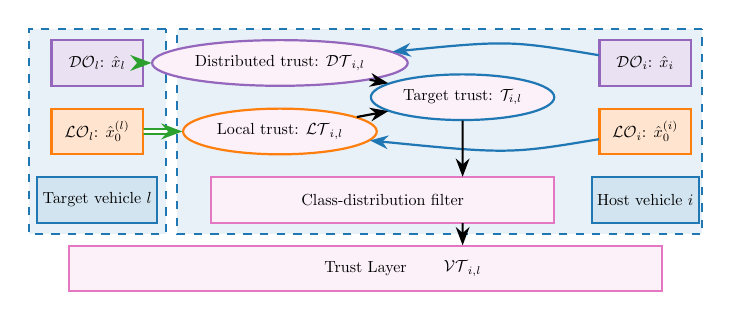
\begin{tikzpicture}[global scale = 0.58,
    vehicle/.style={draw=blue1, fill=blue1!20, thick, minimum width=2cm, minimum height=1cm},
    localobs/.style={draw=orange1, fill=orange1!20, thick, minimum width=2cm, minimum height=1cm},
    distobs/.style={draw=purple1, fill=purple1!20, thick, minimum width=2cm, minimum height=1cm},
    sigarrow/.style={-Stealth, thick, color=blue1},
    commarrow/.style={
    double,
    double distance=1pt,
    line width=0.7pt,
    draw=green1,
    -Stealth
    },
    physics/.style={draw=blue1, shape=rectangle, fill=blue1!10,line width=0.75pt,dashed,minimum width=3cm, minimum height=4.5cm}, %
    trustlayer/.style={draw=rose1, shape=rectangle, fill=rose1!10,thick,minimum width=13cm, minimum height=1cm},
    trust/.style={draw=rose1, shape=ellipse, fill=rose1!10,thick,minimum width=1.5cm, minimum height=1cm}
]

        \node[physics,line width=0.75pt,minimum width=3cm, minimum height=4.5cm] at(2,1.5) { };
        \node[vehicle, name=target] at(2,0) {Target vehicle $l$};
        \node[localobs, name=LOt] at(2,1.5) {$\LO_{l}$: $\hat{x}_{0}^{(l)}$};
        \node[distobs, name=DOt] at(2,3) {$\DO_{l}$: $\hat{x}_{l}$};

        \node[physics,line width=0.75pt,minimum width=11.5cm, minimum height=4.5cm,name=host] at(9.5,1.5) {};
        \node[vehicle,name=host] at(14,0) {Host vehicle $i$};
        \node[localobs,name=LOh] at(14,1.5) {$\LO_{i}$: $\hat{x}_{0}^{(i)}$};
        \node[distobs,name=DOh] at(14,3) {$\DO_{i}$: $\hat{x}_{i}$};

        \node[trust,draw = purple1, name=DT] at(6,3) {Distributed trust: $\DT_{i,l}$};
        \node[trust,draw = orange1, name=LT] at(6,1.5) {Local trust:  $\LT_{i,l}$};
        \node[trust,draw = blue1, name=T] at(10,2.25) {Target trust: $\T_{i,l}$};

        \node[trust,shape=rectangle,name=evo, minimum width=7.5cm] at(8.25,0) {Class-distribution filter};
        \node[name=evo,minimum height=1cm] at(10,0) {};

        \node[trustlayer] at(0.5/2+15.25/2,-1.5) {Trust Layer};
        \node[name = VT,minimum height=1cm] at(10,-1.5) {$\VT_{i,l}$};

        \draw[commarrow] (DOt) -- (DT);
        \draw[commarrow] (LOt) -- (LT);

        \draw[sigarrow] (LOh) .. controls +(-3,-0.5).. (LT);
        \draw[sigarrow] (DOh) .. controls +(-3,0.5).. (DT);

        \draw[sigarrow, black] (LT) -- (T);
        \draw[sigarrow,black] (DT) -- (T);

        \draw[sigarrow,black] (T) -- (evo);
        \draw[sigarrow,black] (evo) -- (VT);
    \end{tikzpicture}
    \caption{Trust framework.}
    \label{fig_trust_framework}
\end{figure}

\subsection{Packet validity gate}\label{subsec_packet_gate}
Before any behavioral trust score is computed, host $i$ checks whether the received V2V packet from source $l$ is authenticated and fresh:
{\small
\begin{equation}
    g_{i,l}^{\mathrm{pkt}}(t)=
    \begin{cases}
        1, & \text{if the message is authenticated and fresh}, \\
        0, & \text{otherwise.}
    \end{cases}
\end{equation}
}
The packet gate is a prerequisite for trust evaluation rather than a trust score by itself. When $g_{i,l}^{\mathrm{pkt}}(t)=0$, the current packet is not used to form new consistency indicators, and the corresponding trust states are aged according to their decay laws. When $g_{i,l}^{\mathrm{pkt}}(t)=1$, the packet enters the local and distributed trust computations below.

\subsection{Local trust}\label{sub:local_trust}
Local trust evaluates the physical consistency of the source's local-observer anchor packet with information available at the host. For accepted packets, let $r_{i,l}^{\mathrm{meas}}$ and $v_{i,l}^{\mathrm{rel,meas}}$ be host-side relative position and speed, and $\hat p_0^{(l)}=[\hat X_0^{(l)},\hat Y_0^{(l)}]^\top$. Then
\begin{align*}
    r_{i,l}^{\mathrm{obs}}(t)
    &=
    \begin{bmatrix}
    \hat X_0^{(l)}(t)-\hat X_0^{(i)}(t)\\
    \hat Y_0^{(l)}(t)-\hat Y_0^{(i)}(t)
    \end{bmatrix},\\
    \Delta\hat p_0^{(l)}(t)&=\hat p_0^{(l)}(t)-\hat p_0^{(l)}(t-1),\\
    \psi_{l}^{\mathrm{pos}}(t)&=
    \mathrm{atan2}\big(\Delta\hat Y_0^{(l)}(t),\Delta\hat X_0^{(l)}(t)\big).
\end{align*}
The planar position, speed, and heading consistency indicators are
\begin{align}
    \iota_{i,l}^{\mathrm{pos}}
    &=
    \max\left(
    1-
    \frac{\left\|r_{i,l}^{\mathrm{obs}}-r_{i,l}^{\mathrm{meas}}\right\|}
    {\varepsilon_p+\left\|r_{i,l}^{\mathrm{meas}}\right\|},0
    \right), \notag\\
    \iota_{i,l}^{\mathrm{speed}}
    &=
    \max\left(
    1-
    \frac{\left|(\hat v_{0}^{(l)}-\hat v_{0}^{(i)})-v_{i,l}^{\mathrm{rel,meas}}\right|}
    {\varepsilon_v+\left|v_{i,l}^{\mathrm{rel,meas}}\right|},0
    \right), \notag\\
    \iota_{i,l}^{\mathrm{heading}}
    &=
    \max\left(
    1-
    \frac{\left|\mathrm{wrap}_{\pi}(\hat\psi_0^{(l)}-\psi_l^{\mathrm{pos}})\right|}
    {\varepsilon_{\psi}+\psi_{\mathrm{th}}},0
    \right),
    \label{eq_local_consistency_indicators}
\end{align}
where $\varepsilon_p,\varepsilon_v>0$ and $\psi_{\mathrm{th}}>0$. The heading factor is omitted when $\|\Delta\hat p_0^{(l)}\|$ is below a motion threshold; any unavailable factor is likewise omitted, avoiding $0^0$. With exponents $\omega_p,\omega_v,\omega_\psi\ge0$, the raw local trust is
\begin{align}
    \LT_{i,l}^{\mathrm{raw}}(t)
    &=
    \left(\iota_{i,l}^{\mathrm{pos}}(t)\right)^{\omega_p}
    \left(\iota_{i,l}^{\mathrm{speed}}(t)\right)^{\omega_v}
    \notag\\
    &\quad\times
    \left(\iota_{i,l}^{\mathrm{heading}}(t)\right)^{\omega_\psi}.
    \label{eq_local_trust_product}
\end{align}
Invalid or missing packets are handled by decay:
\begin{equation}
    \LT_{i,l}(t) =
    \left\{ \begin{array}{ll}
        \LT_{i,l}^{\mathrm{raw}}(t),  &  \text{if } g_{i,l}^{\mathrm{pkt}}(t) = 1, \\
        (1 - \lambda_h)\LT_{i,l}(t-1), & \text{otherwise,}
    \end{array}\right.
    \label{eq_local_trust_update}
\end{equation}
where $\lambda_h\in[0,1]$ sets the loss-decay rate.

\subsection{Distributed trust}
Distributed Trust checks the exchanged fleet estimate against three residuals: sender self-consistency, agreement with the host estimate, and agreement with host-side relative measurements:
\begin{equation}
        \DT_{i,l}(t)  = \begin{cases}
       \gamma_{i,l}^{\text{self}}(t)\gamma_{i,l}^{\text{local}}(t)
       \gamma_{i,l}^{\text{host}}(t),   &  g_{i,l}^{\mathrm{pkt}}(t) = 1, \\
        (1 - \lambda_h)\DT_{i,l}(t-1), & \text{otherwise}.
    \end{cases}
\end{equation}
Let $\|z\|_M^2=z^\top M z$. The sender self-consistency factor is
\begin{equation}
    \gamma_{i,l}^{\text{self}}(t)
    =
    \exp\left(
    -\|\hat{x}_l^{(l)}(t)-\hat{x}_0^{(l)}(t)\|_{\Sigma_{\text{self}}^{-1}}^2
    \right).
\end{equation}
The host-estimate residuals are
\begin{align}
    \mu_{i,l}^{(j)}(t)
    &=
    \|\hat{x}_i^{(j)}(t)-\hat{x}_l^{(j)}(t)\|_{\Sigma_{\text{host}}^{-1}}^2,
    \label{eq_dis_glo}\\
    D_{i,l}^{\text{host}}(t)
    &=
    \sum_{j=1}^N \mu_{i,l}^{(j)}(t), \qquad
    \gamma_{i,l}^{\text{host}}(t)
    =
    \exp\left(-D_{i,l}^{\text{host}}(t)\right),
\end{align}
where $n=4$ and $\Sigma_{\text{host}}=\diag{\sigma_1^2,\ldots,\sigma_n^2}$ is estimated from nominal discrepancies. Let $y_{i,j}\in\mathbb{R}^{m_{ij}}$ be a relative measurement and $H_{ij}$ its selection matrix. 
Suppressing time arguments,
\begin{align}
    \varepsilon_{i,l}^{(j)}
    &=
    H_{ij}\left(\hat{x}_l^{(j)}-\hat{x}_l^{(i)}\right)-y_{i,j}, \notag\\
    E_{i,l}(t)
    &=
    \sum_{j\in\N_i}
    \|\varepsilon_{i,l}^{(j)}(t)\|_{\Sigma_{\ell,ij}^{-1}}^2,\qquad
    \gamma_{i,l}^{\text{local}}(t)
    =
    \exp\left(-E_{i,l}(t)\right).
\end{align}
All covariance matrices are positive definite receiver-side quantities calibrated from nominal data.

\subsection{Target trust and temporal evolution}\label{subsec_evolution}
The instantaneous target trust combines local and distributed consistency:
\begin{equation}
    \T_{i,l}(t) =  \LT_{i,l}(t) \cdot \DT_{i,l}(t).
    \label{trs_sample_genral}
\end{equation}
Because $\T_{i,l}(t)$ can change abruptly, the observer uses a smoothed Vehicle Trust $\VT_{i,l}(t)$. Let $q=5$ denote the ordered classes \textit{Unreliable}, \textit{Poor}, \textit{Acceptable}, \textit{Good}, and \textit{Excellent}. Their scores and intervals are
\begin{equation}
    \kappa_m=\frac{m-1}{q-1}, \qquad m=1,\ldots,q,
\end{equation}
\begin{equation}
    \mathcal{I}_m =
    \begin{cases}
    \left[\dfrac{m-1}{q},\dfrac{m}{q}\right), & m=1,\ldots,q-1,\\[1ex]
    \left[\dfrac{q-1}{q},1\right], & m=q.
    \end{cases}
\end{equation}
The current score is mapped to a one-hot class vector and accumulated as
\begin{equation}
    r_{i,l,m}(t)=
    \begin{cases}
    1, & \T_{i,l}(t)\in \mathcal{I}_m,\\
    0, & \text{otherwise,}
    \end{cases}
    \qquad
    r_{i,l}(t)\in\mathbb{R}^{q}.
\end{equation}
\begin{equation}
    R_{i,l}(t+1)=
    \left(1-\beta_{\text{trust}}\T_{i,l}(t)\right)R_{i,l}(t)
    +r_{i,l}(t),
    \label{eq_class_history_update}
\end{equation}
where $\beta_{\text{trust}}\in[0,1]$, $R_{i,l}(0)\ge0$, and $\alpha_{\mathrm{tr}}\ge0$ satisfies $\mathbf1_q^\top\alpha_{\mathrm{tr}}=1$. With confidence $C_{\mathrm{tr}}>0$, define
\begin{equation}
    S_{i,l,m}(t)=
    \frac{R_{i,l,m}(t)+C_{\mathrm{tr}}\alpha_{\mathrm{tr},m}}
    {C_{\mathrm{tr}}+\sum_{s=1}^{q}R_{i,l,s}(t)},
    \qquad m=1,\ldots,q.
    \label{eq_class_distribution}
\end{equation}
\begin{equation}
    \VT_{i,l}(t)=
    \sum_{m=1}^{q}\kappa_m S_{i,l,m}(t).
    \label{eq_class_filtered_vehicle_trust}
\end{equation}
This is a discounted finite-class Dirichlet mean~\cite{josang2007dirichlet}; larger $\beta_{\text{trust}}$ reacts faster, whereas larger $C_{\mathrm{tr}}$ strengthens the prior.

\subsection{Practical parameter selection}\label{subsec_trust_tuning}
The trust parameters are selected from nominal data: $\Omega_z$ from physical limits, covariance matrices from an attack-free window, and trust thresholds and memory from nominal validation. The resulting weights are checked against Section~\ref{sec_weight_design}.


% For the controller interface, each host vehicle also forms an opinion vector
% \begin{equation}
%     \O_i(t)=[\O_i(1,t),\ldots,\O_i(N,t)],
% \end{equation}
% where $\O_i(i,t)=1$ and $\O_i(l,t)=\VT_{i,l}(t)$ for trusted neighbors. For non-neighboring vehicles, $\O_i(j,t)$ can be obtained from one-hop propagated opinions or assigned a conservative default when no credible propagated opinion is available. This vector is used only as a compact reliability summary for the controller blending factor in Section~\ref{sec_simulation}; the observer-weight design below uses the pairwise trust values directly.

\section{Trust-Based Observer Weight Design}\label{sec_weight_design}
The trust framework provides each vehicle with smoothed vehicle-trust scores $\VT_{i,l}(t)$ representing the reliability of information from other vehicles.
Fix a rejection threshold $\theta_{\min}\in(0,1]$. Throughout this section, $\|\cdot\|_*$ denotes a fixed norm on the bicycle state space, and all induced and block norms are formed from this same state norm unless stated otherwise.
This section shows how the trust values define adaptive observer weights $w_{il}^{(j)}(t)$ and establishes conditions for stability of the estimation error dynamics.

\subsection{Trust-based weights}
Using the virtual graph $\bar{\G}^{(j)}$, each vehicle $i$ first selects the trusted neighbor sources at time $t$:
\begin{equation}
\mathcal{LN}^{(j)}_{i}(t)
= \Big\{l\in\N_i\mid g_{i,l}^{\mathrm{pkt}}(t)=1,\;
\VT_{i,l}(t)\ge\theta_{\min}\Big\}.
\end{equation}
The selected trust scores are then used directly as reliability scores,
\begin{align}
s_{i,l}^{(j)}(t)
&=
\begin{cases}
\VT_{i,l}(t), & l\in\mathcal{LN}^{(j)}_{i}(t),\\
0, & \text{otherwise},
\end{cases}
\label{new_setneibor}\\
S_i^{(j)}(t)
&=\epsilon+\sum_{r\in\N_i}s_{i,r}^{(j)}(t),
\end{align}
where $\epsilon>0$ avoids division by zero. Let $\eta_0,\eta_N\in[0,1]$ denote the local-anchor and neighbor-consensus budgets, respectively, with
\begin{equation}
    \eta_0+\eta_N\le1 .
\end{equation}
Let $\chi_{i0}^{(j)}(t)\in\{0,1\}$ indicate that the local-anchor packet $\hat{x}_0^{(j)}(t)$ is available and accepted at host $i$. For the target's own host, $\chi_{j0}^{(j)}(t)=1$ and $\LT_{j,j}(t)=1$; if the anchor packet is unavailable or rejected, $\chi_{i0}^{(j)}(t)=0$ and the anchor weight is zero. The local-anchor weight is
\begin{equation}\label{eq_anchor_weight}
w_{i0}^{(j)}(t)=
\begin{cases}
\eta_0\chi_{i0}^{(j)}(t)\LT_{i,j}(t), &
\substack{\chi_{i0}^{(j)}(t)=1,\\ \LT_{i,j}(t)\ge\theta_{\min},}\\
0, & \text{otherwise},
\end{cases}
\end{equation}
and the neighbor weights are
\begin{equation}\label{design_gain}
    w_{il}^{(j)}(t)
    =
    \eta_N
    \frac{s_{i,l}^{(j)}(t)}
    {S_i^{(j)}(t)},
    \qquad l\in\N_i .
\end{equation}
Thus, rejected neighbors receive zero weight, while accepted neighbors share at most the budget $\eta_N$ in proportion to their trust values. The remaining mass is the implicit self-prediction weight
\begin{equation}
    w_{is}^{(j)}(t)
    =
    1-w_{i0}^{(j)}(t)-\sum_{l\in\N_i}w_{il}^{(j)}(t).
\end{equation}

The weight law is an admissible nonnegative mixture.

\begin{lemma}[Admissibility of trust weights]\label{lem_weight_admissible}
The weight law~\eqref{new_setneibor}--\eqref{design_gain} satisfies $w_{il}^{(j)}(t)\ge0$, $w_{i0}^{(j)}(t)\ge0$, and
\begin{equation}
\sum_{l\in\N_i\cup\{0\}}w_{il}^{(j)}(t)\le1
\end{equation}
for all $i,j$ and all $t$.
\end{lemma}
\begin{proof}
All reliability scores are nonnegative and $S_i^{(j)}(t)>0$, so $w_{il}^{(j)}(t)\ge0$. The anchor satisfies $0\le w_{i0}^{(j)}(t)\le\eta_0$, and the neighbor budget satisfies
\[
\sum_{l\in\N_i}w_{il}^{(j)}(t)
=\eta_N\frac{\sum_{l\in\N_i}s_{i,l}^{(j)}(t)}
{\epsilon+\sum_{l\in\N_i}s_{i,l}^{(j)}(t)}
\le\eta_N .
\]
Hence the total correction mass is at most $\eta_0+\eta_N\le1$.
\end{proof}

The lemma provides bounded mixing, but bounded mixing alone is not sufficient for convergence because the bicycle model contains prediction dynamics. The accepted trust-induced weights must also provide enough local-anchor mass, or enough rooted multi-step information flow, to contract the distributed prediction error. Let
\begin{equation}
    M^{(j)}(t)=I_N-\bar{\L}^{(j)}(t).
\end{equation}
By Lemma~\ref{lem_weight_admissible}, $M^{(j)}(t)$ is nonnegative and its $i$th row sum is $1-w_{i0}^{(j)}(t)$. Therefore, in the infinity norm,
\begin{equation}
    \|M^{(j)}(t)\|_{\infty}
    =
    \max_{i\in\V}\big(1-w_{i0}^{(j)}(t)\big).
    \label{eq_M_inf_norm}
\end{equation}
The proposed weight law gives a direct lower bound on this missing row mass whenever the target-local anchor packet is accepted.

\begin{lemma}[Anchor-induced one-step contraction]\label{lem_anchor_contraction}
Suppose that, for target $j$, the accepted anchor packet is available to every host at time $t$ and satisfies $\chi_{i0}^{(j)}(t)=1$ and $\LT_{i,j}(t)\ge\theta_{\min}$ for all $i\in\V$. Then the weight law~\eqref{eq_anchor_weight} gives
\begin{equation}
    w_{i0}^{(j)}(t)\ge \underline w_0,
    \qquad
    \underline w_0:=\eta_0\theta_{\min} .
\end{equation}
Consequently,
\begin{equation}
    \|M^{(j)}(t)\|_{\infty}\le 1-\underline w_0.
\end{equation}
If the bicycle map is Lipschitz on the admissible compact region in the same state norm with constant $L_{x,j}$ and
\begin{equation}
    L_{x,j}\big(1-\underline w_0\big)<1,
    \label{eq_anchor_contraction_check}
\end{equation}
then the homogeneous distributed prediction error is a one-step contraction.
\end{lemma}
\begin{proof}
Under the stated acceptance condition,~\eqref{eq_anchor_weight} gives $w_{i0}^{(j)}(t)=\eta_0\LT_{i,j}(t)\ge\eta_0\theta_{\min}$. The row-sum identity~\eqref{eq_M_inf_norm} then gives $\|M^{(j)}(t)\|_{\infty}\le1-\underline w_0$. Combining this with~\eqref{eq_nonlinear_lipschitz} yields the contraction factor in~\eqref{eq_anchor_contraction_check}.
\end{proof}

When direct anchors are intermittent, the same argument must be applied over a window. These weights induce a switching communication graph because the trusted-neighbor set changes online. A plain union spanning tree is not enough unless the anchor information can move through the matrix product in time order. We therefore use the following sequential rooted accepted-graph condition, where an edge $l\to i$ means that the accepted weight $w_{il}^{(j)}$ is positive.
\begin{assumption}[Sequentially rooted accepted graph]\label{ass_graph}
There exist $T_c>0$ and $\underline w\in(0,1]$ such that, for every $j,t$, and $i$, an ordered temporal path $v_0=0,v_1,\ldots,v_m=i$ occurs at $t\le\tau_1<\cdots<\tau_m\le t+T_c-1$. Every path-edge weight and every implicit self weight that carries the path influence between $\tau_1$ and the window end is at least $\underline w$.
\end{assumption}
Thus every host receives target-anchor influence through an accepted time-ordered path; an unordered union spanning tree alone is insufficient.

\begin{lemma}[Rooted block contraction]\label{lem_rooted_block_contraction}
If Assumption~\ref{ass_graph} holds, then the grounded trust-mixing product satisfies
\begin{equation}
    \left\|
    M^{(j)}(t+T_c-1)\cdots M^{(j)}(t)
    \right\|_{\infty}
    \le 1-\underline w^{T_c} .
    \label{eq_grounded_product_bound}
\end{equation}
Let $L_{x,j}(\tau)\le L_{x,j}$ be a scalar one-step Lipschitz bound that applies uniformly to all hosts estimating target $j$ at time $\tau$. For the separable interleaved prediction--mixing estimate below, define
\begin{equation}
    G_{x,j}(T_c)
    :=\sup_{t\ge0}\prod_{r=0}^{T_c-1}L_{x,j}(t+r)
    \le L_{x,j}^{T_c}.
\end{equation}
When time-resolved bounds are unavailable, the conservative choice is $G_{x,j}(T_c)=L_{x,j}^{T_c}$. The one-step gains are scalar and therefore factor through the mixing matrices. For the componentwise error-size vector
\begin{equation}\label{eq_E}
E^{(j)}(t)=\col{\|e_1^{(j)}(t)\|_*,\ldots,\|e_N^{(j)}(t)\|_*},
\end{equation}
the one-step homogeneous recursion satisfies, componentwise,
\begin{equation}
E^{(j)}(t+1)
\le L_{x,j}(t)M^{(j)}(t)E^{(j)}(t).
\end{equation}
Unrolling this recursion over one block gives
\begin{align}
E^{(j)}(t+T_c)
&\le G_{x,j}(T_c)
\big(M^{(j)}(t+T_c-1)\cdots M^{(j)}(t)\big)\notag\\
&\quad\times E^{(j)}(t).
\label{eq_componentwise_block_bound}
\end{align}
Thus $G_{x,j}(T_c)$ is an upper bound for the product of the one-step gains in every admissible interleaved block; it is not an independently chosen gain for the prediction-only composition. This explains why the scalar prediction gain and the trust-mixing product separate. If
\begin{equation}
    G_{x,j}(T_c)\big(1-\underline w^{T_c}\big)
    \le \alpha_c<1,
    \label{eq_window_contraction_check}
\end{equation}
then the distributed homogeneous error is contractive over every window of length $T_c$. The one-step condition~\eqref{eq_anchor_contraction_check} is the special case $T_c=1$ with direct anchor acceptance at every step.
\end{lemma}
\begin{proof}
Let $P_r=M^{(j)}(t+r-1)\cdots M^{(j)}(t)$ and $d_r=\mathbf1-P_r\mathbf1$. Since $\mathbf1-M^{(j)}(\tau)\mathbf1=w_0^{(j)}(\tau)$,
\[
d_{r+1}=w_0^{(j)}(t+r)+M^{(j)}(t+r)d_r.
\]
Along each path in Assumption~\ref{ass_graph}, this recursion transfers and preserves a deficit of at least $\underline w^{T_c}$ to the destination row. Hence $P_{T_c}\mathbf1\le(1-\underline w^{T_c})\mathbf1$, proving~\eqref{eq_grounded_product_bound};~\eqref{eq_componentwise_block_bound} then gives~\eqref{eq_window_contraction_check}.
\end{proof}

Thus, contraction is not assumed from trust scoring alone. The weight law supplies the anchor lower bound through $\eta_0\theta_{\min}$ when anchor packets are directly accepted, and Assumption~\ref{ass_graph} supplies the corresponding lower bound for sparse or intermittent trusted paths. If all reliable paths to a target are rejected, the theorem applies only to the reachable part of the platoon, and that target cannot be reconstructed from communication alone.

\subsection{Observer design procedure}
The design steps are:
\begin{enumerate}
    \item Fix $\Omega_x\times\Omega_u$ and compute $L_{x,j},L_{u,j}$.
    \item Choose $F_j(t)$ and verify~\eqref{eq_ltv_lyapunov}; with $C_j=I_4$, $F_j=A_j$ makes the linearized error matrix zero.
    \item Compute trust, acceptance variables, and weights from~\eqref{eq_anchor_weight}--\eqref{design_gain}.
    \item Check~\eqref{eq_anchor_contraction_check} or~\eqref{eq_window_contraction_check}; otherwise mark the target uncertified or unreachable.
\end{enumerate}

\subsection{Stability of the error}\label{subsec_Prove}
For target $j$, let $e_0^{(j)}=\hat x_0^{(j)}-x_j$, $e_i^{(j)}=\hat x_i^{(j)}-x_j$, and $e_{\DO}^{(j)}=\col{e_1^{(j)},\ldots,e_N^{(j)}}$. The local and distributed nonlinear error recursions induced by~\eqref{eq_LO} and~\eqref{eq_DO} are
\begin{align}
e_0^{(j)}(t+1)
&=f_{\mathrm b}(\hat x_0^{(j)},u_j)
+F_j\big(y_j-h_j(\hat x_0^{(j)})\big)-x_j(t+1),
\label{eq_raw_e0}\\
e_i^{(j)}(t+1)
&=f_{\mathrm b}(\hat x_{i,c}^{(j)},\hat u_j)-x_j(t+1),\quad i\in\V,
\label{eq_raw_eDO}
\end{align}
where $\hat x_{i,c}^{(j)}$ is the trust-weighted correction in~\eqref{eq_consensus_state}; time arguments on its right-hand side are omitted for readability.
\begin{assumption}[Compact operating region]\label{ass_compact_region}
The trajectories considered in the analysis remain in a compact set $\Omega_x\times\Omega_u$ with bounded speed and inputs, $|\delta|\le\delta_{\max}<\pi/2$, accepted packets inside the receiving-side admissible set~\eqref{eq_received_packet_gate}, and a local yaw chart without wrap discontinuities.
\end{assumption}
Under Assumption~\ref{ass_compact_region}, there are finite $L_{x,j},L_{u,j}>0$ such that
\begin{equation}
\begin{aligned}
\|f_{\mathrm b}(\xi,\mu)-f_{\mathrm b}(\zeta,\nu)\|_*
&\le L_{x,j}\|\xi-\zeta\|_*
+L_{u,j}\|\mu-\nu\|_*
\end{aligned}
\label{eq_nonlinear_lipschitz}
\end{equation}
for all $(\xi,\mu),(\zeta,\nu)\in\Omega_x\times\Omega_u$. Conservative Lipschitz bounds and the local gain are computed from the trajectory Jacobians
\begin{align}
 A_i(t)&=\left.\frac{\partial f_{\mathrm b}}{\partial x}\right|_{(\bar x_i,\bar u_i)},\quad
 B_i(t)=\left.\frac{\partial f_{\mathrm b}}{\partial u}\right|_{(\bar x_i,\bar u_i)},\notag\\
 C_i(t)&=\left.\frac{\partial h_i}{\partial x}\right|_{\bar x_i}=I_4.
 \label{eq_bicycle_jacobian}
\end{align}

Throughout the distributed-error analysis, we use the block maximum norm
\begin{equation}
\|e_{\DO}^{(j)}(t)\|_{\mathrm{b},*}
:=\max_{i\in\V}\|e_i^{(j)}(t)\|_* .
\label{eq_block_max_norm}
\end{equation}
The same block-norm convention is used for other stacked state vectors below.
By Lemma~\ref{lem_weight_admissible}, $M^{(j)}(t)=I_N-\bar\L^{(j)}(t)$ is entrywise nonnegative and its $i$th row sum is $1-w_{i0}^{(j)}(t)$. Component-wise, its entries follow from the grounded Laplacian:
\begin{equation}
M_{ik}^{(j)}(t)=
\begin{cases}
w_{is}^{(j)}(t), & k=i,\\
w_{ik}^{(j)}(t), & k\neq i,\; k\in\N_i,\\
0, & \text{otherwise},
\end{cases}
\label{eq_mixing_entries}
\end{equation}
where $w_{is}^{(j)}(t)$ is the implicit self-prediction weight. The $i$th row sum is therefore $w_{is}^{(j)}(t)+\sum_{k\in\N_i}w_{ik}^{(j)}(t)=1-w_{i0}^{(j)}(t)$. Nonnegativity allows the triangle inequality to pass through the weighted correction. For every host $i$,
\begin{align}
\left\|\sum_{k=1}^N {M_{ik}^{(j)}(t)}e_k^{(j)}(t)\right\|_*
&\le \sum_{k=1}^N M_{ik}^{(j)}(t)\|e_k^{(j)}(t)\|_*\notag\\
&\le \big(1-w_{i0}^{(j)}(t)\big)
\|e_{\DO}^{(j)}(t)\|_{\mathrm{b},*}.
\label{eq_rowwise_mixing_bound}
\end{align}
Taking the maximum over $i$ yields the induced mixing norm $\|M^{(j)}(t)\|_\infty=\max_i(1-w_{i0}^{(j)}(t))$ used in the contraction arguments.

Stacking the trust-weighted correction and using the nonnegative row-substochastic weights gives
\begin{align}
\|e_{c,\DO}^{(j)}(t)\|_{\mathrm{b},*}
&\le \|M^{(j)}(t)\|_\infty
\|e_{\DO}^{(j)}(t)\|_{\mathrm{b},*}\notag\\
&\quad+\|w_0^{(j)}(t)\|_\infty\|e_0^{(j)}(t)\|_*
+\|r_{\mathrm{chart}}^{(j)}(t)\|_{\mathrm{b},*} ,
\label{eq_nonlinear_consensus_bound}
\end{align}
where $M^{(j)}=I_N-\bar\L^{(j)}$, $w_0^{(j)}$ stacks the anchor weights, and $r_{\mathrm{chart}}^{(j)}$ is zero in the no-wrap Euclidean chart (or a bounded second-order retraction remainder).

The Jacobians in~\eqref{eq_bicycle_jacobian} provide the usual auxiliary linearized model for selecting $F_j$ and checking conservative contraction constants, but the result below is stated for the nonlinear recursions~\eqref{eq_raw_e0}--\eqref{eq_raw_eDO}.

If $a_0^{(j)}$ and $a_l^{(j)}$ corrupt the anchor and neighbor-$l$ channels, respectively, the correction at host $i$ contains
{\small
\begin{equation}
\xi_{\mathrm{att},i}^{(j)}(t)
=w_{i0}^{(j)}(t)a_{0}^{(j)}(t)
+\sum_{l\in\mathcal{M}_{i}^{(j)}(t)}w_{il}^{(j)}(t)a_{l}^{(j)}(t).
\label{eq_attack_input}
\end{equation}
}
Here $\mathcal{M}_i^{(j)}(t)\subseteq\N_i$ denotes the corrupted neighbor channels seen by host $i$ for target $j$; for unattacked, unavailable, or rejected channels the corresponding attack vector is zero.

By~\eqref{eq_nonlinear_lipschitz}, this perturbation enters the nonlinear error recursion as an additive ISS input bounded by
\begin{equation}
\|d_{\mathrm{att},i}^{(j)}(t)\|_*
\le L_{x,j}\|\xi_{\mathrm{att},i}^{(j)}(t)\|_* .
\label{eq_attack_lipschitz_bound}
\end{equation}
Stacking these row-wise terms gives the additive input $d_{\mathrm{att}}^{(j)}$. Its size is modulated by the trust weights.
If $\|a_{0}^{(j)}(t)\|_*\le \bar a_0$ and $\|a_{l}^{(j)}(t)\|_*\le \bar a_{\mathrm{N}}$ on $\mathcal{M}_{i}^{(j)}(t)$, then Lemma~\ref{lem_weight_admissible} gives
\begin{align}
\|d_{\mathrm{att},i}^{(j)}(t)\|_*
&\le L_{x,j}
\left(
w_{i0}^{(j)}(t)\bar a_0
+\sum_{l\in\mathcal{M}_{i}^{(j)}(t)}
w_{il}^{(j)}(t)\bar a_{\mathrm{N}}
\right) \notag\\
&\le L_{x,j}\max\{\bar a_0,\bar a_{\mathrm{N}}\}.
\label{eq_attack_bound}
\end{align}
Thus $\|d_{\mathrm{att}}^{(j)}(t)\|_{\mathrm{b},*}\le\bar d_{\mathrm{att}}$ for some finite $\bar d_{\mathrm{att}}$; after rejection, the corrupted channel's direct term in~\eqref{eq_attack_input} is zero.

For the nonlinear ISS proof, $d_0^{(j)}$ and $d_{\DO}^{(j)}$ denote the corresponding lumped inputs caused by model uncertainty, input mismatch, chart remainders, and bounded approximation terms. We assume these inputs and the additive attack contribution are bounded.
\begin{assumption}\label{assum_distur}
There are finite $\bar d_0$, $\bar d_{\DO}$, and $\bar d_{\mathrm{att}}$ such that, for every $t$, $\|d_0^{(j)}(t)\|_*\le\bar d_0$, $\|d_{\DO}^{(j)}(t)\|_{\mathrm{b},*}\le\bar d_{\DO}$, and $\|d_{\mathrm{att}}^{(j)}(t)\|_{\mathrm{b},*}\le\bar d_{\mathrm{att}}$. Hence $\|\tilde d_{\DO}^{(j)}(t)\|_{\mathrm{b},*}\le\bar{\tilde d}_{\DO}:=\bar d_{\DO}+\bar d_{\mathrm{att}}$.
\end{assumption}

\begin{lemma}[Local nonlinear observer ISS]\label{lem_local_iss}
Assume that, on $\Omega_x\times\Omega_u$, the disturbance-free local nonlinear error recursion associated with~\eqref{eq_raw_e0} is uniformly locally exponentially stable with constants $c_{\ell}>0$ and $\lambda_{\ell}\in(0,1)$. Then, for sufficiently small initial errors and bounded local inputs, the perturbed recursion remains in a local invariant neighborhood and is ISS. In particular, for some finite local input gain $\gamma_{\ell}>0$,
\begin{equation}
\|e_0^{(j)}(t)\|_*
\le c_{\ell}\lambda_{\ell}^{t}\|e_0^{(j)}(0)\|_*
+\gamma_{\ell}\bar d_0 .
\label{eq_local_iss_bound}
\end{equation}
A sufficient check is the uniform exponential stability of the LTV local-error recursion
\begin{equation}
z(t+1)=\big(A_j(t)-F_j(t)C_j(t)\big)z(t),
\label{eq_ltv_local_error}
\end{equation}
understood as an LTV system, not as frozen-time Schur stability. It is enough to find bounded $P_j(t)=P_j(t)^\top$ and scalars $0<\underline p\le\bar p$, $q>0$ such that, with $A_{F,j}(t):=A_j(t)-F_j(t)C_j(t)$,
\begin{align}
\underline p\, I \preceq P_j(t)\preceq\bar p I,\notag\\
A_{F,j}(t)^\top P_j(t+1)A_{F,j}(t)-P_j(t)
\preceq-qI
\label{eq_ltv_lyapunov}
\end{align}
for all $t$, with a sufficiently small invariant neighborhood where the nonlinear remainder is uniformly quadratic.
\end{lemma}
\begin{proof}
Uniform local exponential stability gives a local Lyapunov function with quadratic bounds and a strict one-step decrease. In a small invariant neighborhood, the additive input perturbs this decrease by a term proportional to $\|d_0^{(j)}\|_*$. Iterating the comparison inequality and using Assumption~\ref{assum_distur} gives~\eqref{eq_local_iss_bound}. The LTV Lyapunov inequality~\eqref{eq_ltv_lyapunov} is a checkable way to establish the required uniform exponential stability before accounting for the quadratic nonlinear remainder.
\end{proof}

\begin{lemma}[Nonlinear distributed-error contraction]\label{lem_dist_contraction}
Suppose that the block contraction condition~\eqref{assume3} below holds. If the local-observer error is ISS and Assumption~\ref{assum_distur} holds, then the nonlinear distributed error~\eqref{eq_raw_eDO} is ISS with respect to $e_0^{(j)}$ and $d_{\DO}^{(j)}$. Under the additive attack model, the attacked distributed error is ISS with respect to $e_0^{(j)}$ and $\tilde d_{\DO}^{(j)}$.
\end{lemma}
\begin{proof}
With the componentwise error-size vector $E^{(j)}(t)$ in~\eqref{eq_E}, the Lipschitz bound~\eqref{eq_nonlinear_lipschitz}, the row-wise mixing bound~\eqref{eq_rowwise_mixing_bound}, and the anchor/disturbance terms give
\begin{equation}
E^{(j)}(t+1)
\le L_{x,j}(t)M^{(j)}(t)E^{(j)}(t)+b^{(j)}(t),
\label{eq_componentwise_input_recursion}
\end{equation}
where $\|b^{(j)}(t)\|_\infty$ is bounded by finite gains multiplying $\|e_0^{(j)}(t)\|_*$ and $\|\tilde d_{\DO}^{(j)}(t)\|_{\mathrm{b},*}$. Define
\begin{equation}
\Phi_M^{(j)}(t,T_c)
:=M^{(j)}(t+T_c-1)\cdots M^{(j)}(t).
\label{eq_block_mixing_product}
\end{equation}
Unrolling over a block and using~\eqref{eq_componentwise_block_bound} yields
\begin{align}
\|E^{(j)}(t+T_c)\|_\infty
&\le G_{x,j}(T_c)
\|\Phi_M^{(j)}(t,T_c)\|_\infty
\|E^{(j)}(t)\|_\infty\notag\\
&\quad+c_b\sup_{\tau\in[t,t+T_c-1]}
\|e_0^{(j)}(\tau)\|_*\notag\\
&\quad+c_b\sup_{\tau\in[t,t+T_c-1]}
\|\tilde d_{\DO}^{(j)}(\tau)\|_{\mathrm{b},*}
\label{eq_distributed_block_recursion}
\end{align}
for some finite $c_b>0$. Condition~\eqref{assume3} makes the homogeneous block gain strictly smaller than one. Repeated application of~\eqref{eq_distributed_block_recursion} gives the ISS bound at block times; bounded one-step gains cover intermediate samples, and Lemma~\ref{lem_local_iss} bounds the local-anchor input. In the nominal case, $d_{\mathrm{att}}^{(j)}=0$ and $\tilde d_{\DO}^{(j)}=d_{\DO}^{(j)}$.
\end{proof}

Combining Lemmas~\ref{lem_local_iss} and~\ref{lem_dist_contraction} gives the following result.
\begin{theorem}\label{thm_observer}
Fix a target $j\in\V$. Consider the vehicle platoon~\eqref{eq_platoon} over the directed weighted communication network $\bar{\G}^{(j)}$, and let~\eqref{eq_observer} be the corresponding nonlinear distributed observer for target $j$. Assume that the following conditions hold:
\begin{enumerate}
    \item The local nonlinear error is uniformly locally exponentially stable;~\eqref{eq_ltv_lyapunov} is a sufficient LTV check.
    \item For all $i \in \V$, $w_{i0}^{(j)}(t) \geq 0$ and $w_{il}^{(j)}(t) \geq 0$ satisfy
    \begin{equation}\label{thm_W}%\label{sum_w_il}
    \sum_{l\in \N_i\cup\{0\}} w_{il}^{(j)}(t) \leq 1.
    \end{equation}
    \item There exist a window length $T_c\ge1$ and a scalar $\alpha_c\in(0,1)$ such that, uniformly over all admissible switches, the infinity norm induced by the block maximum norm~\eqref{eq_block_max_norm} satisfies
    \begin{equation} \label{assume3}
    G_{x,j}(T_c)
    \left\|M^{(j)}(t+T_c-1)\cdots M^{(j)}(t)\right\|_\infty
    \le \alpha_c<1.
    \end{equation}
    Here $G_{x,j}(T_c)$ is the separable interleaved block gain defined in Lemma~\ref{lem_rooted_block_contraction}; the conservative choice is $L_{x,j}^{T_c}$. A checkable sufficient condition for $T_c=1$ is Lemma~\ref{lem_anchor_contraction}; for intermittent anchors or sparse accepted graphs, Assumption~\ref{ass_graph} can be enforced by a supervisor or checked on each completed window, and Lemma~\ref{lem_rooted_block_contraction} gives the corresponding block check~\eqref{eq_window_contraction_check}.
\end{enumerate}
Then the original nonlinear error dynamics~\eqref{eq_raw_e0}--\eqref{eq_raw_eDO} are locally ISS on $\Omega_x\times\Omega_u$. Under the additive attack model, the attacked estimation error is also locally ISS. The bounds below hold for sufficiently small initial errors and bounded-input suprema for which the perturbed errors remain in the local invariant neighborhoods of Lemma~\ref{lem_local_iss} and Lemma~\ref{lem_dist_contraction}. In particular, choose any
\begin{equation}
\max\{\alpha_c^{1/T_c},\lambda_{\ell}\}<\lambda<1.
\label{eq_cascade_rate}
\end{equation}
There then exist constants $c_0,c_1>0$ such that
\begin{align}
\|e_0^{(j)}(t)\|_* &\le c_0\lambda^t \|e_0^{(j)}(0)\|_* + c_0 \bar{d}_0,\\
\|e_{\DO}^{(j)}(t)\|_{\mathrm b,*} &\le c_1\lambda^t
\Big(\|e_{\DO}^{(j)}(0)\|_{\mathrm b,*}+\|e_0^{(j)}(0)\|_*\Big)\notag\\
&\quad+c_1\Big(\bar d_0+\bar{\tilde d}_{\DO}\Big).
\end{align}

\end{theorem}
\begin{proof}
Condition~1 and Assumption~\ref{assum_distur} give the local-observer ISS bound by Lemma~\ref{lem_local_iss}. Lemma~\ref{lem_weight_admissible} gives Condition~2 and the nonnegative row-substochastic structure used in~\eqref{eq_rowwise_mixing_bound}. Condition~3 gives the distributed block contraction in Lemma~\ref{lem_dist_contraction}. Substituting~\eqref{eq_local_iss_bound} into the block recursion~\eqref{eq_distributed_block_recursion} produces the convolution of the block rate $\alpha_c^{1/T_c}$ with the local rate $\lambda_{\ell}$. For any $\lambda$ satisfying~\eqref{eq_cascade_rate}, this convolution is bounded by a finite constant times $\lambda^t$, including when the two original rates coincide. The finite within-block, bounded-gain, and norm-equivalence constants are absorbed into $c_0,c_1$, which gives the stated decay of both initial errors and the bounded disturbance terms. In the nominal case $d_{\mathrm{att}}^{(j)}=0$ and $\bar{\tilde d}_{\DO}=\bar d_{\DO}$.
\end{proof}

\begin{remark}
The result is local under Assumption~\ref{ass_compact_region}. The Jacobians in~\eqref{eq_bicycle_jacobian} provide conservative design constants, while the LTV local-error check must be performed along the trajectory rather than through frozen-time eigenvalues alone. Dense accepted-anchor graphs use $T_c=1$; sparse switching graphs use the ordered windows of Assumption~\ref{ass_graph}. Rejection drives the malicious input gain to zero.
\end{remark}

\section{Contamination Rollback Under Delayed Trust Decisions}\label{sec_rollback}
Trust values are computed from consistency windows and therefore may lag behind the first corrupted packet. During this detection delay, falsified data can enter the distributed observer before the corresponding neighbor is removed from the trusted set. To limit this transient contamination, each host vehicle can optionally maintain a finite rollback buffer and re-evaluate the most recent observer steps once a neighbor is flagged.

Each host performs rollback using the data stored in its own buffer. It can remove a rejected source only when data from that source appear directly in the buffer. For example, suppose an attacked vehicle $l^{\star}$ sends false data to vehicle $m$, and vehicle $m$ then sends a contaminated estimate to vehicle $i$. If vehicle $i$ has stored only the estimate from $m$, replaying its buffer cannot identify and remove the contribution of $l^{\star}$.

Correcting this indirect contamination would require either provenance information, meaning a record of the upstream packets and weights used to form each stored estimate, or a coordinated replay in which $m$ corrects its history before $i$ replays its own data. Therefore, the procedure below directly corrects only rejected data contained in the host's own buffer.

Assume that a trust decision is made at time $t$ after the update that produced the pre-reset estimate $\hat{x}_i^{(j)}(t^-)$ and before the reset-corrected estimate at time $t$ is released. Thus, replay over $k=t-K,\ldots,t-1$ produces the replacement value for $\hat{x}_i^{(j)}(t)$. For a rollback horizon $K$, host vehicle $i$ stores, for each observer $\DO_i^{(j)}$ and each time $k\in\{t-K,\ldots,t-1\}$, the pre-update state $\hat{x}_i^{(j)}(k)$, the received neighbor and anchor estimates, the original weights, the input estimate, and the corresponding validity metadata. Let $\mathcal{R}_i^{(j)}(t)\subseteq\N_i$ be the neighbor sources retrospectively rejected by the new decision, let $\chi_{i0,\mathrm r}^{(j)}(k;t)\in\{0,1\}$ denote retrospective acceptance of the archived anchor, and let $\hat u_{j,\mathrm r}(k;t)$ be an archived or recomputed input estimate that remains accepted at replay time. If no accepted bounded input estimate is available, replay is not certified and the target is marked temporarily unavailable. The replay is executed as follows:
\begin{enumerate}
    \item form the retrospective neighbor, anchor, and input acceptance decisions from the trust decision at time $t$;
    \item reset a temporary replay state to the stored state at the beginning of the buffer;
    \item replay the observer from $t-K$ to $t-1$ using only archived channels that remain accepted;
    \item replace the current distributed estimate by the replayed value.
\end{enumerate}
The replay can remove only contributions introduced during the stored interval. Full removal additionally requires the buffer-start state $\hat x_i^{(j)}(t-K)$ to be an unaffected checkpoint; if the first affected packet predates the buffer or the checkpoint is already contaminated, replay is only a bounded mitigation step.

Define the retrospectively masked weights
\begin{align}
\bar w_{il}^{(j)}(k;t)
&=w_{il}^{(j)}(k)\mathbf 1_{\{l\notin\mathcal R_i^{(j)}(t)\}},\quad l\in\N_i,\notag\\
\bar w_{i0}^{(j)}(k;t)
&=w_{i0}^{(j)}(k)\chi_{i0,\mathrm r}^{(j)}(k;t).
\label{eq_rollback_masked_weights}
\end{align}
During replay, the corrected state $x_{\mathrm{r}}$ is used to recompute the innovation terms
\begin{align}
\tilde{\eta}_{il}^{(j)}(k;x_{\mathrm{r}})
&= \bar w_{il}^{(j)}(k;t)
\big(\hat{x}_l^{(j)}(k)-x_{\mathrm{r}}\big),\quad l\in\N_i, \\
\tilde{\eta}_{i0}^{(j)}(k;x_{\mathrm{r}})
&= \bar w_{i0}^{(j)}(k;t)
\big(\hat{x}_0^{(j)}(k)-x_{\mathrm{r}}\big).
\end{align}
The host resets the temporary state to the buffer start,
\begin{equation}
    x_{\mathrm{r}} \leftarrow \hat{x}_i^{(j)}(t-K),
\end{equation}
and replays the observer update for $k=t-K,\ldots,t-1$:
\begin{equation}
\begin{aligned}
x_{\mathrm{r}} \leftarrow\;&
f_{\text{b}}\!\left(
x_{\mathrm{r}}
+\sum_{l\in\N_i}\tilde{\eta}_{il}^{(j)}(k;x_{\mathrm{r}})
+ \tilde{\eta}_{i0}^{(j)}(k;x_{\mathrm{r}}),
\hat{u}_{j,\mathrm r}(k;t)\right).
\end{aligned}
\label{eq_rollback_replay}
\end{equation}
Finally, the current distributed estimate is corrected by setting
\begin{equation}
    \hat{x}_i^{(j)}(t)\leftarrow x_{\mathrm{r}}.
\end{equation}

Because the masked weights in~\eqref{eq_rollback_masked_weights} do not exceed the original weights, their sum remains at most one; the removed weight remains assigned to the replay state through the residual self coefficient, so replay does not require renormalization. The rollback memory cost is proportional to $K\deg(i)$ per observer and can be implemented with archived packets, weights, inputs, and validity metadata. The anchor innovation is retained only when its archived channel remains accepted.

\begin{lemma}[Bounded rollback reset]\label{lem_rollback_bounded}
Assume that the stored packets, masked weights, accepted inputs, replayed states, and pre-reset estimates remain in the compact admissible region used in Theorem~\ref{thm_observer}, and that the rollback horizon $K$ is finite. At a reset time $\tau_q$, define the stacked reset $\zeta_{\DO}^{(j)}(\tau_q)$ by stacking
\[
    \zeta_i^{(j)}(\tau_q)=x_{\mathrm r}-\hat{x}_i^{(j)}(\tau_q^-)
\]
for the resetting hosts and zeros for the other hosts. Then $\|\zeta_{\DO}^{(j)}(\tau_q)\|_{\mathrm{b},*}\le\bar\zeta$ for some finite $\bar\zeta$. Suppose also that every post-reset error remains in the local invariant neighborhood of Theorem~\ref{thm_observer}, and that $\tau_{q+1}-\tau_q\ge T_{\mathrm r}$ for an integer $T_{\mathrm r}\ge1$. Let $C_{\mathrm r}>0$ and $\rho_{\mathrm r}\in(0,1)$ bound the reset-free homogeneous distributed-error transition, as supplied by the block contraction condition. If $\mathcal B_{\mathrm{ISS}}^{(j)}(t)$ denotes the reset-free ISS bound of Theorem~\ref{thm_observer}, including norm-equivalence constants, then
\begin{align}
\|e_{\DO}^{(j)}(t)\|_{\mathrm{b},*}
&\le \mathcal B_{\mathrm{ISS}}^{(j)}(t)
+C_{\mathrm r}\!\sum_{\tau_q<t}\rho_{\mathrm r}^{\,t-\tau_q}
\|\zeta_{\DO}^{(j)}(\tau_q)\|_{\mathrm{b},*}\notag\\
&\le \mathcal B_{\mathrm{ISS}}^{(j)}(t)
+\frac{C_{\mathrm r}\bar\zeta}{1-\rho_{\mathrm r}^{T_{\mathrm r}}}.
\label{eq_rollback_iss_bound}
\end{align}
Thus the reset-augmented observer is locally practically ISS with respect to the ordinary disturbances and the rollback-reset sequence.
\end{lemma}
\begin{proof}
For fixed finite $K$, the replay map is a finite composition of bounded weighted corrections and bicycle predictions on a compact set. It is therefore bounded. Since the pre-reset estimate is also bounded in the same admissible region, the difference between the replayed state and the pre-reset estimate is bounded, which gives a finite $\bar\zeta$. Between reset times, the block contraction proof of Theorem~\ref{thm_observer} gives a transition bound $C_{\mathrm r}\rho_{\mathrm r}^{t-s}$. Inserting each reset as an additive jump and iterating this bound gives the first inequality in~\eqref{eq_rollback_iss_bound}. The integer separation of reset times bounds the resulting geometric series by $(1-\rho_{\mathrm r}^{T_{\mathrm r}})^{-1}$, which gives the second inequality. The post-reset neighborhood condition ensures that the local estimates used in this iteration remain valid.
\end{proof}
Lemma~\ref{lem_rollback_bounded} proves boundedness of the reset-augmented error; it does not guarantee that every rollback decreases the estimation error. Error reduction depends on a sufficiently early unaffected checkpoint and on correct retrospective channel decisions.

\subsection{Pose propagation and relative-measurement re-anchoring}
Rollback mitigates short-term contamination caused by delayed trust decisions. In contrast, re-anchoring provides an independent pose reference that limits the long-term propagation of accumulated position offsets when a trusted anchor or accepted relative measurement is available. This distinction separates ordinary pose propagation from optional relative-measurement re-anchoring.


Let $p=[X,Y]^\top$ and write the consensus-corrected state as
$\hat{x}_{i,c}^{(j)}=\col{\hat p_{i,c}^{(j)},\hat\psi_{i,c}^{(j)},\hat v_{i,c}^{(j)}}$.
The usual observer prediction propagates the corrected pose as
\begin{equation}
    \hat p_i^{(j)}(t+1)
    =
    \hat p_{i,c}^{(j)}(t)
    +T_s\hat v_{i,c}^{(j)}(t)
    \begin{bmatrix}
        \cos \hat\psi_{i,c}^{(j)}(t)\\
        \sin \hat\psi_{i,c}^{(j)}(t)
    \end{bmatrix}.
    \label{eq_pose_propagation}
\end{equation}
Equation~\eqref{eq_pose_propagation} is a motion update, not a position reset. If $\hat p_{i,c}^{(j)}$ is biased by contaminated cooperative data, then clean velocity or heading only gives a cleaner motion vector from a biased starting point. The position offset remains.

Re-anchoring is an optional correction before prediction. If host vehicle $i$ has an onboard relative measurement to target $j$, and this measurement passes the same validity and trust checks used in the local-trust layer, then the host can build an independent pose reference for $j$. With the measured relative position expressed in the global frame,
\begin{equation}
    p_{\mathrm{rel},i}^{(j)}(t)
    =
    \hat p_0^{(i)}(t)+r_{i,j}^{\mathrm{meas}}(t),
    \label{eq_relative_pose_anchor}
\end{equation}
where $\hat p_0^{(i)}$ is the host local-observer position and $r_{i,j}^{\mathrm{meas}}$ is the measured relative position from $i$ to $j$. This reference does not come from the received distributed estimate of target $j$; it comes from host sensing and the host's own local pose.

The host may then blend the corrected base pose with this relative-measurement reference:
\begin{equation}
\begin{aligned}
    p_{\mathrm b,i}^{(j)}(t)
    &=
    \big(1-\rho_{i,\mathrm{rel}}^{(j)}(t)\big)\hat p_{i,c}^{(j)}(t)
    +\rho_{i,\mathrm{rel}}^{(j)}(t)p_{\mathrm{rel},i}^{(j)}(t),
    \\
    \rho_{i,\mathrm{rel}}^{(j)}(t)&\in[0,1],
\end{aligned}
    \label{eq_pose_reanchor_base}
\end{equation}
and predict from the resulting base pose,
\begin{equation}
    \hat p_i^{(j)}(t+1)
    =
    p_{\mathrm b,i}^{(j)}(t)
    +T_s \hat v_{i,c}^{(j)}(t)
    \begin{bmatrix}
        \cos \hat\psi_{i,c}^{(j)}(t)\\
        \sin \hat\psi_{i,c}^{(j)}(t)
    \end{bmatrix}.
    \label{eq_pose_reanchor_prediction}
\end{equation}
Here $\rho_{i,\mathrm{rel}}^{(j)}=0$ gives the proved observer and $\rho_{i,\mathrm{rel}}^{(j)}=1$ resets the pose base. Missing or rejected relative data set $\rho_{i,\mathrm{rel}}^{(j)}=0$. The experiments with $\rho_{i,\mathrm{rel}}^{(j)}>0$ are an add-on outside Theorem~\ref{thm_observer}.



\section{Simulation and Platform Results}\label{sec_simulation}

This section reports three validation layers. The numerical campaign uses a five-vehicle platoon and compares local, global, and simultaneous local--global corruption to evaluate RMSE, trust response, source suppression, and the dominant attack cases. The QCar/LIMO validation then checks rollback under real packet timing and uses trajectories to show closed-loop path effects. Finally, the control check uses trust as a gate between CACC and ACC and verifies positive projected spacing during the attack interval.

\subsection{Numerical Simulation Setup}

The numerical study considers a five-vehicle platoon with all-to-all V2V communication. Each vehicle runs the proposed observer, and small fixed parameter variations are treated as modeling uncertainty. The main simulation parameters are $N=5$, $T_s=0.01$~s, nominal geometry $l_f=1.11$~m and $l_r=1.74$~m, giving $L_w=2.85$~m, local-trust product fusion with internal powers $(\omega_p,\omega_v,\omega_\psi,\omega_u)=(2.0,3.0,1.0,1.0)$ for distance/position, velocity, heading, and acceleration/input consistency, class-filter aging weight $\beta_{\text{trust}}=0.45$ in the active single-rating update, class confidence $C_{\mathrm{tr}}=0.2$, $q=5$ trust classes, heading base tolerance $\psi_{\mathrm{th}}=0.35$~rad, and trust threshold $\theta_{\min}=0.5$. The observer-weight module uses base gains $w_{0,\mathrm{base}}=0.4$ and $w_{\mathrm{self,base}}=0.2$, with nominal neighbor budget $0.4$ and per-neighbor cap $0.4$. After trust gating and flag normalization, these quantities define adaptive fusion weights rather than fixed lower bounds.

For the direct-anchor case of Theorem~\ref{thm_observer}, the contraction check uses the scaled infinity norm $\|z\|_*=\|D_xz\|_\infty$, with $D_x=\mathrm{diag}(0.01,0.01,1,0.2)$, to account for mixed state units. On the operating set $v\le33$~m/s and $|\delta|\le0.35$~rad, the induced one-step bicycle gain is $L_{x,\max}\approx1.007$. With accepted anchor mass $\underline w_0=\eta_0\theta_{\min}=0.20$, Lemma~\ref{lem_anchor_contraction} gives $\alpha=L_{x,\max}(1-\underline w_0)\approx1.007\times0.80\approx0.806<1$. This verifies the distributed direct-anchor condition; the local condition uses the full-state choice in Step~2 above. If a target anchor is rejected, reconstruction from communication alone is not claimed; the implementation holds or marks the estimate as temporarily unreachable until an accepted anchored path returns.

\subsection{Evaluation Metrics}
Let $\mathcal K_{\mathrm{att}}=\{k:10\le kT_s\le15\}$ and $q\in\{d,v,a\}$, where $\hat a$ is the input-estimator output. For non-attacker targets,
\begin{equation}
\operatorname{RMSE}_{q,i}=
\sqrt{\frac{1}{|\mathcal K_{\mathrm{att}}|}\sum_{k\in\mathcal K_{\mathrm{att}}}
\left(q_i(k)-\hat q_i(k)\right)^2}.
\end{equation}
The raw combined RMSE used for ranking is
\begin{equation}
S_{\mathrm{raw},i}
=\operatorname{RMSE}_{d,i}+\operatorname{RMSE}_{v,i}
+\operatorname{RMSE}_{a,i}.
\end{equation}
Because $S_{\mathrm{raw}}$ mixes units, it is only a within-campaign index. Detection is the first mean attacker trust below $\theta_{\mathrm{op}}=0.70$; trust drop and source zero-rate respectively measure credibility loss and the fraction of zero attacker-source weights.

\subsection{Attack Scenarios}\label{sec:attack_scenarios}
The numerical campaign uses a single corrupted source in a five-vehicle platoon. The corrupted vehicle is V1, and V2--V5 are the non-attacker targets used in the RMSE summaries. Each attack is active on $[10,15]$~s. Table~\ref{tab:attack_mix} lists five concrete instances of the threat model in Section~\ref{subsec_threat_model}: Cases~1--4 are FDI-type corruptions of the communicated bicycle state, and Case~5 is a DoS-type packet-drop corruption. Replay/delay is not assigned a separate numerical ID because stale packets are handled by the timestamp/freshness gate; the delayed-decision effect is instead evaluated in the QCar/LIMO rollback tests below.

The same five attacks are evaluated under three channel-corruption modes. In a local-channel attack, the corrupted source falsifies the local-anchor packet $\hat{x}_0^{(1)}$ broadcast by V1. In a global-channel attack, it falsifies V1's broadcast fleet estimate $\hat{x}_1$. In the simultaneous local--global attack, both packet types are corrupted over the same time window. This separation matches the observer architecture in Section~\ref{sec_distributed_observer} and keeps the channel comparison under identical attack amplitudes.

\begin{table}[!ht]
\centering
\caption{Five bicycle-state attack IDs used in the numerical campaign.}
\label{tab:attack_mix}
\scriptsize
\begin{tabular}{p{0.7cm}p{1.35cm}p{2.0cm}p{3.0cm}}
\toprule
\textbf{Case} & \textbf{Type} & \textbf{Target} & \textbf{Parameters} \\
1 & Bias & Position $X$ & bias = $-5$~m \\
2 & Faulty & Position $X$ & std. = 10~m, $p = 0.5$ \\
3 & Bias & Speed $v$ & bias = $-2.5$~m/s \\
4 & Faulty & Speed $v$ & std. = 2.5~m/s, $p = 0.5$ \\
5 & Drop & All state packets & $p_\text{drop} = 0.5$ \\
\bottomrule
\end{tabular}
\end{table}

\subsection{Numerical Simulation Results}

All attacks are evaluated over the 10--15~s attack window using the raw combined RMSE $S_{\mathrm{raw}}$. Table~\ref{tab:attack_mode_rmse_summary} compares the three corruption modes. Global corruption gives the lowest mean raw combined RMSE, $0.393$, and the lowest dispersion, with standard deviation $0.069$. Local corruption gives the highest average degradation, with mean raw combined RMSE $0.643$. Simultaneous local--global corruption gives an intermediate mean RMSE of $0.567$, but it creates the most severe single residual, $S_{\mathrm{raw}}=3.856$ on V5 under Case~2. The trust-drop column measures how much the mean trust assigned to the corrupted source decreases from the pre-attack baseline to the attack-window average; larger values indicate stronger trust penalization. The source zero-rate is a suppression measure: it is the fraction of attacker-source fusion weights that are set to zero during the attack window, excluding direct self-weight. Thus, a larger source zero-rate means the corrupted source is more often completely removed from distributed fusion.

\begin{table}[!t]
\centering
\caption{Aggregate attack-window performance by corruption mode.}
\label{tab:attack_mode_rmse_summary}
\footnotesize
\setlength{\tabcolsep}{0pt}
\renewcommand{\arraystretch}{1.22}
\begin{tabular*}{\columnwidth}{@{\extracolsep{\fill}}lcccccc@{}}
\toprule
\textbf{Mode} & \shortstack{\textbf{Mean}\\$S_{\mathrm{raw}}$} & \shortstack{\textbf{Std.}\\\textbf{dev.}} & \shortstack{\textbf{Max.}\\$S_{\mathrm{raw}}$} & \shortstack{\textbf{Trust}\\\textbf{drop}} & \shortstack{\textbf{Source}\\\textbf{zero}} & \shortstack{\textbf{Detect.}\\\textbf{time}} \\
\midrule
Local  & $0.643$ & $0.586$ & $2.058$ & $0.319$ & $80.64\%$ & $10.088$~s \\
Global & $0.393$ & $0.069$ & $0.546$ & $0.460$ & $92.90\%$ & $10.028$~s \\
Both   & $0.567$ & $0.796$ & $3.856$ & $0.544$ & $98.44\%$ & $10.030$~s \\
\bottomrule
\end{tabular*}
\vspace{0.9ex}
\parbox{\columnwidth}{\footnotesize\emph{Note:} Std. dev. denotes standard deviation; trust drop is pre-attack attacker trust minus attack-window attacker trust; source zero denotes the attacker-source zero-rate; detection time is the mean first-threshold-crossing time.}
\end{table}

Table~\ref{tab:case_ranking} ranks the attack cases by the mean raw combined RMSE averaged over the three corruption modes. Case~2, the intermittent $10$~m $X$ fault, is the dominant attack: its cross-mode mean is $1.232$, and its RMSE reaches $1.775$ for local corruption, $0.515$ for global corruption, and $1.406$ for simultaneous corruption. The other four cases stay below $0.405$ RMSE in all three configurations.

\begin{table}[!t]
\centering
\caption{Attack-case severity ranking by mean raw combined RMSE.}
\label{tab:case_ranking}
\scriptsize
\setlength{\tabcolsep}{0pt}
\renewcommand{\arraystretch}{1.18}
\begin{tabular*}{\columnwidth}{@{\extracolsep{\fill}}ccclccc@{}}
\toprule
\textbf{Rank} & \textbf{Case} & \textbf{Mean} & \textbf{Attack} & \textbf{Local} & \textbf{Global} & \textbf{Both} \\
\midrule
\textbf{1} & \textbf{2} & $\mathbf{1.232}$ & \textbf{$X$ fault, $10$~m} & $\mathbf{1.775}$ & $\mathbf{0.515}$ & $\mathbf{1.406}$ \\
2 & 4 & $0.387$ & $v$ fault, $2.5$~m/s & $0.361$ & $0.405$ & $0.396$ \\
3 & 3 & $0.363$ & $v$ bias, $-2.5$~m/s & $0.364$ & $0.362$ & $0.362$ \\
4 & 5 & $0.354$ & DoS & $0.380$ & $0.347$ & $0.335$ \\
5 & 1 & $0.334$ & $X$ bias, $-5$~m & $0.334$ & $0.334$ & $0.334$ \\
\bottomrule
\end{tabular*}
\end{table}

The quantitative comparison shows three clear patterns. First, global corruption reduces mean RMSE by $38.9\%$ relative to local corruption. Second, simultaneous local--global corruption is $11.8\%$ lower than local corruption but $44.2\%$ higher than global corruption. Third, simultaneous corruption creates the largest single RMSE, $3.856$, which is $87.4\%$ higher than the local maximum and $7.06$ times the global maximum. Detection reaches $100\%$ in all cases and configurations. The average detection times are close to the $10$~s attack onset, except local Case~4, where the mean detection time is delayed to $10.263$~s. Therefore, local corruption causes the largest average estimation error, global corruption is least damaging on average, and simultaneous local--global corruption creates the highest worst-case outlier risk.

\subsection{QCar/LIMO Platform Rollback and Closed-Loop Trajectory Diagnostics}\label{sec:qcar_limo_platform}

\subsubsection{Platform and Communication Stack}

The observer is also implemented on a mixed QCar/LIMO 1:10 scale platform, where each vehicle runs the same estimation, communication, and control stack under real sensor timing, packet exchange, and controller execution. Vehicles broadcast local estimates, fleet estimates, trust summaries, and packet status. The receiving host checks physical and temporal consistency, updates trust weights, and runs the distributed observer with the local observer as an anchor. The numerical campaign uses labels V1--V5, whereas platform logs use V0, V1, and V2.

Figure~\ref{fig:qcar_limo_scheme} summarizes this flow: peer vehicles exchange UDP packets, the trust observer converts consistency checks into adaptive fusion weights, and the fleet estimate is used for validation and control. The rollback comparison uses the existing cooperative controller; the spacing check uses the trust-blended cooperative/local implementation. The same attack channel supports matched no-rollback and rollback runs.

\begin{figure*}[!t]
    \centering
    \resizebox{\textwidth}{!}{%
    \begin{tikzpicture}[
        font=\scriptsize,
        >=Stealth,
        panel/.style={draw, rounded corners=3pt, line width=0.6pt, align=center, inner sep=0pt},
        module/.style={draw, rounded corners=2pt, fill=white, align=center, minimum height=0.95cm, inner sep=2pt},
        badge/.style={draw, rounded corners=2pt, align=center, minimum height=0.48cm, inner sep=1.5pt, font=\tiny\bfseries},
        paneltitle/.style={font=\footnotesize\bfseries, anchor=north},
        flow/.style={->, thick, shorten >=1.4pt, shorten <=1.0pt},
        exchange/.style={<->, thick, shorten >=1.4pt, shorten <=1.0pt},
        feedback/.style={->, thick, dashed, shorten >=1.4pt, shorten <=1.0pt},
        flowbus/.style={thick, shorten >=1.0pt, shorten <=1.0pt},
        flowlabel/.style={draw=black!20, fill=white, rounded corners=1pt, inner xsep=2pt, inner ysep=1pt, font=\tiny\bfseries}
    ]
        \node[panel, draw=black!45, fill=black!2, minimum width=3.20cm, minimum height=5.35cm, anchor=north west] (platformPanel) at (0,6.25) {};
        \node[paneltitle] at (1.60,6.08) {Platform};
        \node[draw=black!70, rounded corners=2pt, inner sep=0pt, anchor=north] at (1.60,5.55)
            {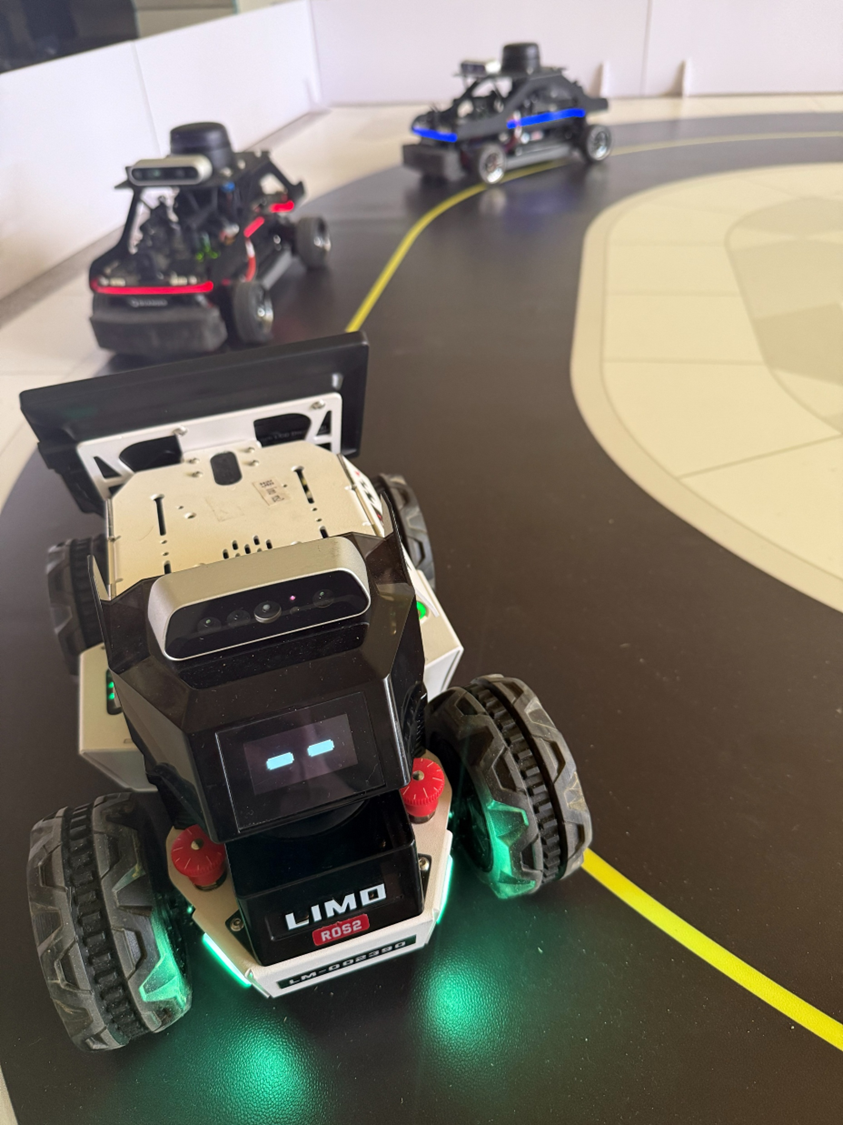
\includegraphics[width=2.60cm,height=3.72cm,keepaspectratio]{img/image.png}};

        \node[panel, draw=userblue, fill=userblue!6, minimum width=2.85cm, minimum height=5.35cm, anchor=north west] (hostPanel) at (3.50,6.25) {};
        \node[paneltitle] at (4.93,6.08) {1. Host Stack};
        \node[module, draw=userblue, text width=2.20cm, minimum width=2.38cm] (sensors) at (4.93,5.05)
            {\textbf{Sensors}\\GPS, IMU, encoder\\camera, input};
        \node[module, draw=userblue, text width=2.20cm, minimum width=2.38cm] (localobs) at (4.93,3.68)
            {\textbf{Local Observer}\\$\hat{x}_i=[X,Y,\psi,v]$\\host estimate};
        \node[module, draw=userblue, text width=2.20cm, minimum width=2.38cm] (logic) at (4.93,2.28)
            {\textbf{Vehicle Logic}\\observer schedule\\telemetry, control};
        \draw[flow, userblue] (sensors) -- (localobs);
        \draw[flow, userblue] (localobs) -- (logic);

        \node[panel, draw=userorange, fill=userorange!7, minimum width=2.85cm, minimum height=5.35cm, anchor=north west] (v2vPanel) at (6.95,6.25) {};
        \node[paneltitle] at (8.38,6.08) {2. V2V Exchange};
        \node[module, draw=userorange, dashed, rounded corners=4pt, text width=2.05cm, minimum width=2.28cm, minimum height=1.28cm] (udp) at (8.38,4.95)
            {\textbf{UDP Network}\\local state\\fleet estimate\\trust report};
        \node[module, draw=userred, fill=userred!6, text width=2.05cm, minimum width=2.28cm, minimum height=0.90cm] (attack) at (8.38,3.45)
            {\textbf{Attack Module}\\false data\\delay/dropout};
        \node[module, draw=userorange, text width=2.05cm, minimum width=2.28cm] (peers) at (8.38,2.05)
            {\textbf{Peer Vehicles}\\same stack on\\each vehicle};
        \draw[flow, userred] (attack.north) -- (udp.south);
        \draw[flow, userred] (attack.south) -- (peers.north);

        \node[panel, draw=userpurple, fill=userpurple!7, minimum width=3.55cm, minimum height=5.35cm, anchor=north west] (trustPanel) at (10.20,6.25) {};
        \node[paneltitle] at (11.98,6.08) {3. Trust Observer};
        \node[module, draw=userpurple, text width=2.88cm, minimum width=3.10cm] (trusteval) at (11.98,5.03)
            {\textbf{Trust Evaluation}\\consistency checks\\quality and timing gates};
        \node[module, draw=userpurple, text width=2.88cm, minimum width=3.10cm, minimum height=1.05cm] (weights) at (11.98,3.58)
            {\textbf{Adaptive Fusion Weights}\\direct, self, neighbor terms\\threshold and influence cap};
        \node[module, draw=userpurple, text width=2.88cm, minimum width=3.10cm, minimum height=1.08cm] (distobs) at (11.98,2.05)
            {\textbf{Distributed Estimation}\\trust-weighted correction\\prediction and rollback};
        \draw[flow, userpurple] (trusteval) -- (weights);
        \draw[flow, userpurple] (weights) -- (distobs);

        \node[panel, draw=usergreen, fill=usergreen!7, minimum width=2.25cm, minimum height=5.35cm, anchor=north west] (resultsPanel) at (14.25,6.25) {};
        \node[paneltitle] at (15.38,6.08) {4. Results};
        \node[module, draw=usergreen, text width=1.56cm, minimum width=1.78cm] (stateout) at (15.38,5.03)
            {\textbf{Fleet State}\\trajectory\\speed};
        \node[module, draw=usergreen, text width=1.56cm, minimum width=1.78cm] (trustout) at (15.38,3.58)
            {\textbf{Trust Data}\\scores\\weights};
        \node[module, draw=usergreen, text width=1.56cm, minimum width=1.78cm] (validout) at (15.38,2.05)
            {\textbf{Validation}\\plots, RMSE\\attack flags};

        \draw[flow, userorange] ([yshift=0.18cm]localobs.east) -- ++(0.36,0) |- ([yshift=-0.18cm]udp.west);
        \node[flowlabel] at (6.62,4.58) {broadcast};
        \draw[flow, userorange] ([yshift=0.12cm]peers.west) -- ++(-0.42,0) |- ([yshift=-0.18cm]localobs.east);
        \node[flowlabel] at (6.62,3.12) {received};
        \draw[flow, userpurple] (udp.east) -- ([yshift=-0.08cm]trusteval.west);
        \draw[exchange, userpurple] (peers.east) -- (distobs.west);
        \coordinate (resultbuslow) at (13.98,2.05);
        \coordinate (resultbusmid) at (13.98,3.58);
        \coordinate (resultbustop) at (13.98,5.03);
        \draw[flowbus, usergreen] (distobs.east) -- (resultbuslow) -- (resultbustop);
        \draw[flow, usergreen] (resultbustop) -- (stateout.west);
        \draw[flow, usergreen] (resultbusmid) -- (trustout.west);
        \draw[flow, usergreen] (resultbuslow) -- (validout.west);
    \end{tikzpicture}}
    \caption{QCar/LIMO experimental scheme for trust-aware cooperative state estimation. Each vehicle runs a local observer and vehicle-logic loop, exchanges V2V estimates and trust reports, and computes trust-weighted distributed estimates with optional rollback.}
    \label{fig:qcar_limo_scheme}
\end{figure*}

Figure~\ref{fig:qcar_limo_vehicle_structure} separates longitudinal cruise control from lateral cross-track and heading control.
% Both QCar and LIMO vehicles therefore share the normalized $(X,Y,\psi,v)$ interface used for position, velocity, yaw, trust, and rollback-correction histories.

\begin{figure}[!t]
    \centering
    \resizebox{\linewidth}{!}{%
    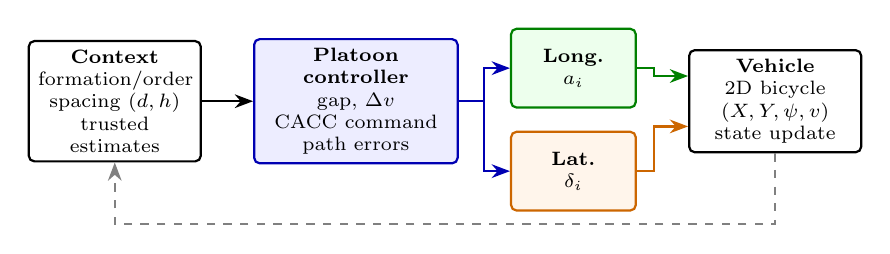
\begin{tikzpicture}[
        font=\scriptsize,
        >=Stealth,
        box/.style={draw, rounded corners=2pt, thick, align=center, minimum height=1.0cm, text width=1.95cm, fill=white},
        ctrl/.style={box, fill=blue!7, draw=blue!70!black, text width=2.35cm},
        cmd/.style={box, fill=green!7, draw=green!50!black, text width=1.35cm},
        lat/.style={box, fill=orange!8, draw=orange!80!black, text width=1.35cm},
        arrow/.style={->, thick},
        fb/.style={->, thick, dashed, gray}
    ]
        \node[box] (context) {
            \textbf{Context}\\
            formation/order\\
            spacing $(d,h)$\\
            trusted estimates
        };

        \node[ctrl, right=0.65cm of context] (controller) {
            \textbf{Platoon controller}\\
            gap, $\Delta v$\\
            CACC command\\
            path errors
        };

        \node[cmd, right=0.65cm of controller, yshift=0.42cm] (long) {
            \textbf{Long.}\\
            $a_i$
        };
        \node[lat, below=0.28cm of long] (lateral) {
            \textbf{Lat.}\\
            $\delta_i$
        };

        \node[box, right=0.65cm of long, yshift=-0.42cm] (vehicle) {
            \textbf{Vehicle}\\
            2D bicycle\\
            $(X,Y,\psi,v)$\\
            state update
        };
        \coordinate (vehicleLongIn) at ([yshift=0.32cm]vehicle.west);
        \coordinate (vehicleLatIn) at ([yshift=-0.32cm]vehicle.west);

        \draw[arrow] (context) -- (controller);
        \draw[arrow, blue!70!black] (controller.east) -- ++(0.32,0) |- (long.west);
        \draw[arrow, blue!70!black] (controller.east) -- ++(0.32,0) |- (lateral.west);
        \draw[arrow, green!50!black] (long.east) -- ++(0.22,0) |- (vehicleLongIn);
        \draw[arrow, orange!80!black] (lateral.east) -- ++(0.22,0) |- (vehicleLatIn);
        \draw[fb] (vehicle.south) -- ++(0,-0.9cm) -| (context.south);
    \end{tikzpicture}}
    \caption{Compact QCar/LIMO vehicle-level controller used in the rollback validation. The commands $a_i$ and $\delta_i$ drive the 2D kinematic bicycle model.}
    \label{fig:qcar_limo_vehicle_structure}
\end{figure}

\subsubsection{Rollback Evaluation Protocol}

The platform validation focuses on delayed-decision rollback rather than deterministic RMSE ranking because packet delays, asynchronous sensing, and execution jitter can let corrupted packets enter the observer before trust drops below the rejection threshold. The primary comparison is the same attack configuration without rollback and with finite-window rollback. After delayed detection, the host replays the recent observer window with the corrected trusted-neighbor set. This is mitigation, not perfect attack rejection, because the CACC-only controller may already have reacted to contaminated states.

Diagnostic clean-motion tests are separated from deployable observer operation. Clean-motion replay can use uncorrupted heading and speed in~\eqref{eq_pose_propagation}, but it keeps the estimator's current base position and exposes residual pose contamination. A hard re-anchor through~\eqref{eq_relative_pose_anchor}--\eqref{eq_pose_reanchor_prediction} is realistic only with an accepted onboard relative measurement or another independently validated pose source; re-anchoring to a clean reference that bypasses the attack injector is used only as an ablation/debugging mode. The QCar/LIMO code, resources, and rollback video are provided in the online resources listed in the author footnote.

\subsubsection{Rollback and Anchoring Results}

To isolate rollback and anchoring, Fig.~\ref{fig:rollback_anchoring} compares three runs under the same attack configuration: trust-based estimation without rollback, with rollback, and with rollback plus relative pose anchoring. 
\begin{figure}[!t]
    \centering
    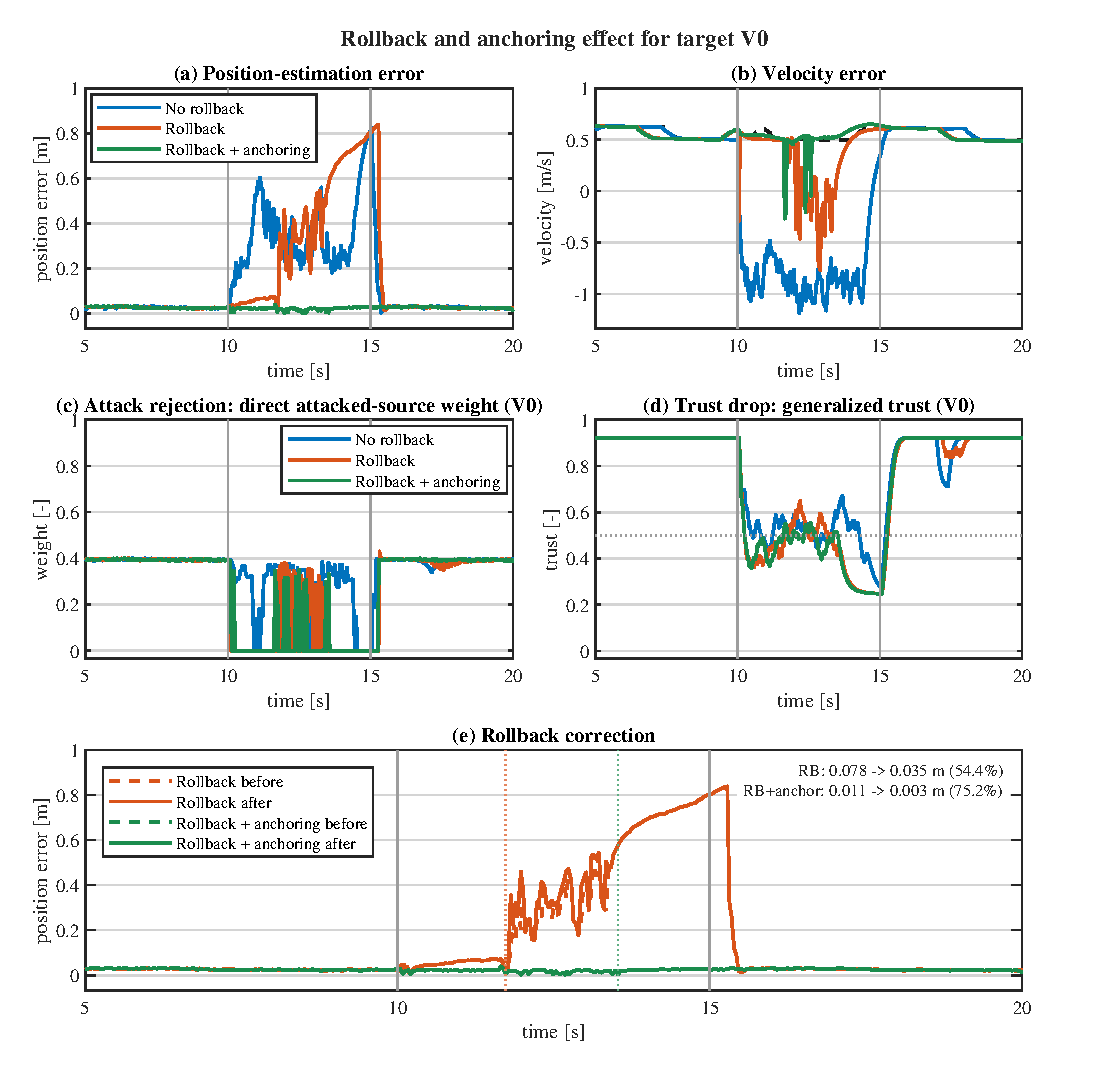
\includegraphics[width=\linewidth]{img/rollback_case3_local.eps}
    \caption{Case 3 local attack on QCar/LIMO: rollback and relative-pose anchoring under real-vehicle delay.}
    \label{fig:rollback_anchoring}
\end{figure}
Figure~\ref{fig:rollback_anchoring} illustrates the response of the trust-based distributed observer when the information used to estimate target vehicle \(V_0\) is compromised. During the attack interval, the observer without rollback accumulates corrupted information, producing a position-estimation error of approximately \(0.8\,\mathrm{m}\) and a pronounced deviation in the estimated velocity. 
The direct attacked-source weight decreases toward zero, indicating that the trust mechanism detects and suppresses the contribution of the compromised source. This behavior is also reflected in the reduction of the generalized trust value during the attack.

Although source rejection prevents further propagation of malicious information, it does not by itself remove the corrupted state already accumulated by the observer. 
The rollback mechanism addresses this limitation by replaying the buffered updates from a stored checkpoint. As shown in Fig.~\ref{fig:rollback_anchoring}(e), rollback reduces the position error by \(54.4\%\) at the correction instant. Introducing anchoring further constrains the reconstructed estimate using accepted relative-pose information, resulting in a \(75.2\%\) error reduction and maintaining the estimation error close to the pre-attack level. In this experiment, the three mechanisms perform complementary functions: rejection suppresses future direct influence from the flagged source, rollback revises its buffered direct contributions, and anchoring improves the consistency of the recovered estimate.
\subsubsection{Closed-Loop Trajectory Diagnostics}

The same platform logs were also replayed as XY trajectory diagnostics. Figures~\ref{fig:XY_case2_local} and~\ref{fig:XY_case2_global} plot the target-\(V_0\) reference, pre-correction estimate, and final estimate for Case~2 local- and global-channel attacks. These plots quantify reconstruction quality on trajectories recorded during closed-loop operation; controller-level effects are assessed separately through the projected-spacing diagnostic below.

\begin{figure}[!t]
    \centering
    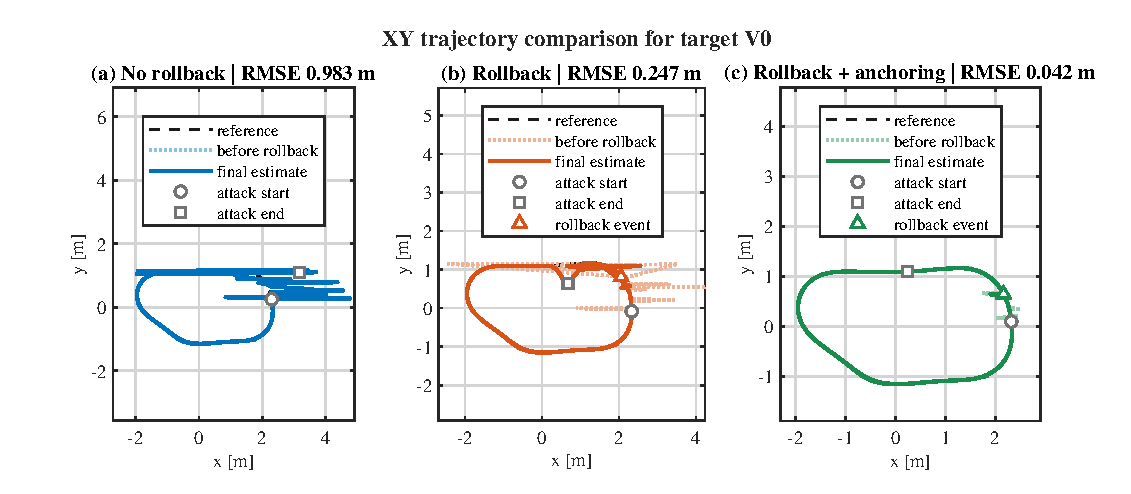
\includegraphics[width=\linewidth]{img/XY_case2_local.eps}
    \caption{Case~2 local-channel XY trajectory reconstruction for target \(V_0\).}
    \label{fig:XY_case2_local}
\end{figure}

\begin{figure}[!t]
    \centering
    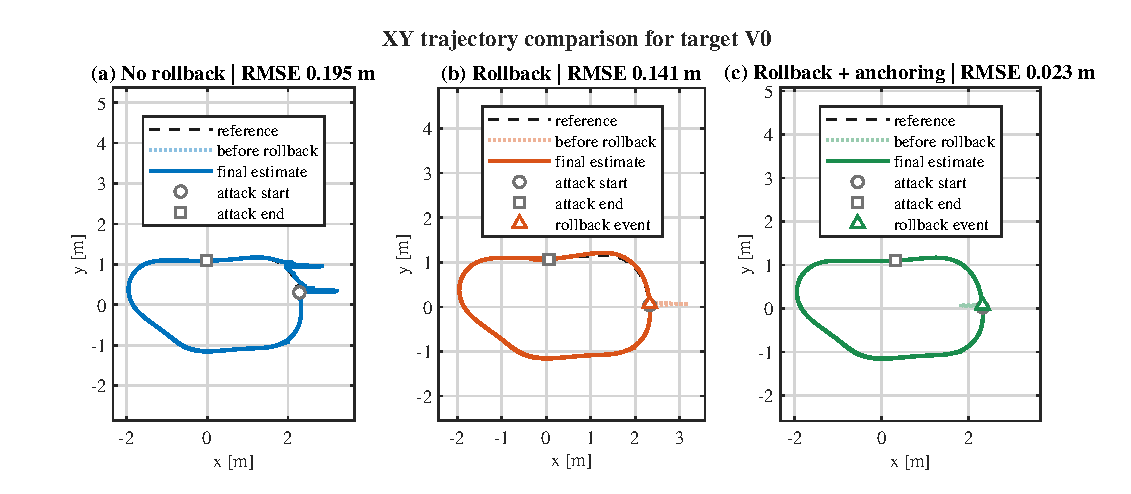
\includegraphics[width=\linewidth]{img/XY_case2_global.eps}
    \caption{Case~2 global-channel XY trajectory reconstruction for target \(V_0\).}
    \label{fig:XY_case2_global}
\end{figure}

In both Case~2 trajectory diagnostics, rollback moves the final estimate closer to the reference, and rollback plus anchoring gives the smallest trajectory RMSE. The plotted RMSE decreases from \(0.983\) to \(0.247\) to \(0.042\)~m in the local-channel run and from \(0.195\) to \(0.141\) to \(0.023\)~m in the global-channel run. The trust and source-suppression behavior for the broader numerical campaign is summarized separately in Table~\ref{tab:attack_mode_rmse_summary}.

\subsection{Distributed State Estimation for Platoon Control}

To complement the estimator validation, this subsection presents an auxiliary idealized closed-loop study. This study is not intended as a standalone control contribution; rather, the longitudinal controller is used as an evaluation layer to examine how the proposed trust-aware estimates may be incorporated into a representative platoon-control architecture. The primary validation remains the estimation and trust-evolution analyses reported above. Under this idealized setting, the longitudinal controller blends local ACC from direct predecessor sensing with CACC based on distributed estimates.

The planar bicycle states are first projected onto the road tangent,
\begin{align}
    e_{\parallel}(k)&=[\cos\psi_{\mathrm{ref}}(k),\sin\psi_{\mathrm{ref}}(k)]^\top,\\
    s_i(k)&=p_i(k)^\top e_{\parallel}(k),
\end{align}
where $p_i=[X_i,Y_i]^\top$ and $\mathcal P_i=\{1,\ldots,i-1\}$ for follower $i\ge2$. Platform V0 corresponds to index 1.


For any attack interval \(\mathcal{K}_{\mathrm{att}}\), define the minimum path-projected bumper-to-bumper spacing
\begin{equation}
    s_{\min}=\min_{k\in\mathcal{K}_{\mathrm{att}}}\min_{i=2,\ldots,N}
    \left((p_{i-1}(k)-p_i(k))^\top e_{\parallel}(k)-L_{\mathrm{veh}}\right),
\end{equation}
where $L_{\mathrm{veh}}$ is vehicle length. In the reported closed-loop replay, this diagnostic is evaluated under the platform \(V_0\) Case~2 attack schedule because Case~2 produced the largest estimation degradation in the numerical campaign. The condition \(s_{\min}>0\) checks positive longitudinal separation along the road tangent, and the \(0.30\)~m threshold is used as an additional reporting margin. This projected-spacing check should not be interpreted as a formal guarantee of full planar vehicle-footprint collision avoidance.

The ACC branch uses the measured predecessor gap and target $d_{\mathrm{ACC}}+h_{\mathrm{ACC}}\max\{\hat v_0^{(i)},0\}$; CACC uses distributed relative errors:
\begin{align}
a_{\mathrm{coop},i}(k)
&= \sum_{j\in\mathcal{P}_i} \big[
    \kappa_s e_{s,ij}(k)
    + \kappa_v e_{v,ij}(k)
    + \kappa_{\psi} e_{\psi,ij}(k)\big],
\end{align}
where $e_{s,ij}$, $e_{v,ij}$, and $e_{\psi,ij}$ are longitudinal-spacing, speed, and wrapped-heading errors, with desired separation $d_{i,j}=(i-j)(d_{\mathrm{ACC}}+h_{\mathrm{ACC}}\hat v_0^{(i)})$. For $\tau_f\in(0,1]$, the command is
\begin{align}
a_{\mathrm{target},i}
&=a_{\mathrm{loc},i}+\gamma_i(a_{\mathrm{coop},i}-a_{\mathrm{loc},i}),\notag\\
\gamma_i&=\VT_{i,i-1},\notag\\
a_i(k)&=a_i(k-1)+\tau_f\big(a_{\mathrm{target},i}(k)-a_i(k-1)\big).
\end{align}
Invalid predecessor packets set $\gamma_i=0$. Therefore, the controller study should be interpreted as a trust-gated ACC/CACC feasibility check with a projected-spacing diagnostic, rather than as a formal string-stability analysis.

\begin{figure}[!t]
    \centering
    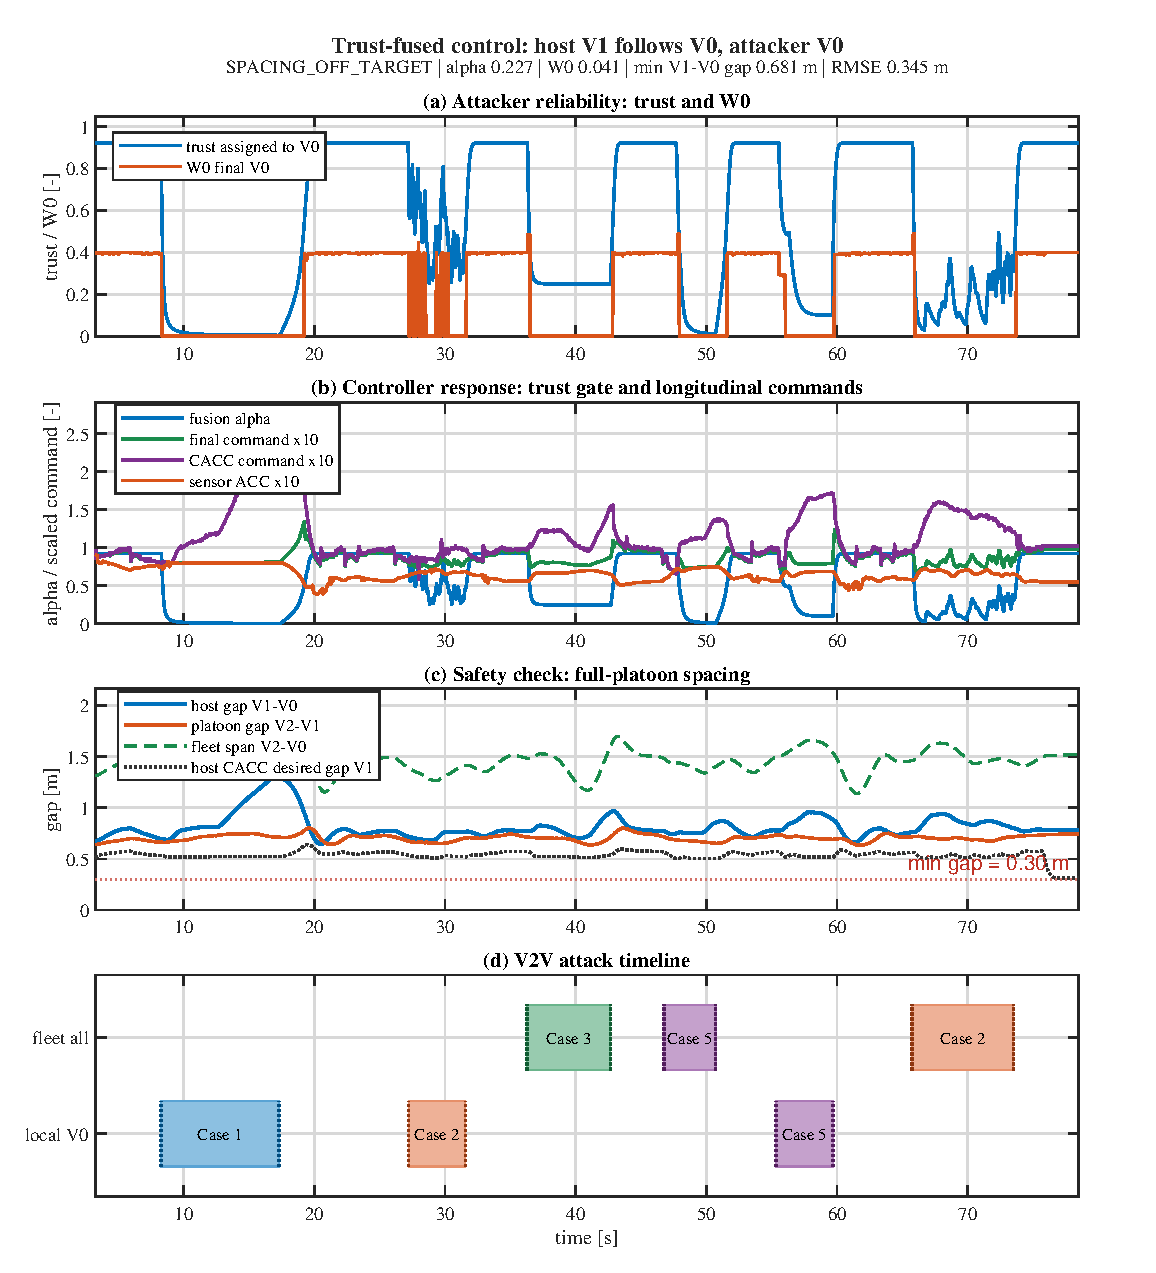
\includegraphics[width=\linewidth]{img/controller_fusion.eps}
    \caption{Trust-gated ACC/CACC response and projected spacing under the platform \(V_0\) attack schedule.}
    \label{fig:controller_fusion}
\end{figure}
\begin{table}[!t]
\centering
\caption{Attack-window closed-loop metrics under the platform \(V_0\) Case~2 attack.}
\label{tab:closed_loop_control_metrics}
\scriptsize
\begin{tabular}{cccccc}
\toprule
Host & $\Delta t_{\mathrm{det}}$ [s] & $\bar{\gamma}_{i,i-1}^{\mathrm{att}}$ & $\bar w_{\mathrm{src}}(V_0)$ & $s_{\min}$ [m] & Gap RMSE [m] \\
\midrule
V1 & 0.093 & 0.227 & 0.041 & 0.681 & 0.345 \\
V2 & 0.090 & 0.894 & 0.048 & 0.637 & 0.171 \\
\bottomrule
\end{tabular}
% \vspace{0.8ex}
\parbox{\linewidth}{\scriptsize\emph{Note:} $\bar{\gamma}_{i,i-1}^{\mathrm{att}}$ is the mean direct-predecessor CACC fusion gate during attacks; $\bar w_{\mathrm{src}}(V_0)$ is the mean observer source weight assigned to the attacked \(V_0\) channel.}
\end{table}

Table~\ref{tab:closed_loop_control_metrics} shows mean attacked-source weight below $0.05$ and minimum projected gaps of $0.681$ and $0.637$~m, both above the $0.30$~m margin.


% Add the closed-loop control figure/table here after running the physical or high-fidelity closed-loop test.
% Suggested report: worst attack case, most affected vehicle i^\star, minimum spacing s_min,
% spacing trajectory, and whether any inter-vehicle distance becomes non-positive.



\section{Discussion and Conclusion}\label{sec_discussion_conclusion}

This paper developed a trust-aware distributed observer for resilient state estimation in connected vehicle platoons. The design combines a local-observer anchor, trust-adaptive fusion weights, and optional finite-window rollback. The anchor prevents drift to a common biased estimate, the trust weights suppress inconsistent neighbors while preserving plausible cooperation, and rollback revises recent updates after delayed trust decisions. The analysis gives sufficient local nonlinear ISS conditions on a compact operating region, covering bounded model uncertainty, input mismatch, accepted corruption, and trust-induced switching. The direct-anchor condition applies when the target anchor is accepted, while the block condition covers intermittent anchors through sequentially rooted accepted graphs.

The guarantee remains conditional. The receiving-side gate~\eqref{eq_received_packet_gate} projects accepted packets onto a physically admissible set, so a large injection is either rejected or converted into a bounded input entering Theorem~\ref{thm_observer} through $\bar d_{\mathrm{att}}$. The result certifies graceful degradation under a specified admissible attack bound, not universal detection or exact reconstruction. A slowly ramping, physically consistent bias inside $\Omega_z$ may still be accepted and leave a nonzero ultimate error. If every accepted anchored path to a target is removed, communication alone cannot reconstruct that target. Rollback is also bounded: it removes only buffered contaminated contributions, assumes a usable checkpoint, and depends on dwell time between resets.

The validation supports these claims within that scope. In simulation, the trust layer detected all injected attacks in the tested campaign and suppressed the corrupted source in most attack-window samples. On the QCar/LIMO platform, rollback recovered much of the delay-induced position error, and the trust-gated ACC/CACC controller maintained positive path-projected spacing for the reported attack schedule. The experiments do not prove formal $f$-resilience, string stability, or full two-dimensional collision avoidance. Future work will focus on stealthy near-threshold attacks, benign false-positive rates, scaled-norm metrics consistent with the $D_x$ contraction check, channel-wise trust, sparse dynamic topologies, post-attack recovery, and closed-loop string stability.


% \IEEEtriggeratref{6}
\bibliographystyle{IEEEtran}
\bibliography{biblio}
\end{document}
